% This file should be replaced with your file with an thesis content.
%=========================================================================
% Authors: Michal Bidlo, Bohuslav Křena, Jaroslav Dytrych, Petr Veigend and Adam Herout 2019


%%%%%%%%%%%%%%%%%%%%%%%%%%%%%%%%%%
% Introduction
\chapter{Introduction}
With the enormous amount of content being published every day, the internet has already become one of the main sources of information for most people in the world. According to Statista\footnote{\url{https://www.statista.com/}}, a German company specializing in market and consumer data, there were approximately 5.16 billion internet users as of January 2023 as stated in \cite{intro-statista1}. This number represents more than 64.4\% of the entire population. The accessibility of information on the internet, however, goes hand in hand with the threat of spreading misinformation and fake news.

Fake news consists of articles intentionally written to convey false information. The purpose of these articles often is to influence and manipulate their audience for their own benefit (e.g., financial, political, etc.). One of the infamous examples of using fake news for manipulation was the 2016 U.S. presidential election where, for instance, the article \cite{intro-pope} quoting "Pope Francis shocks the world, endorses Donald Trump for president, releases a statement." gained over 960,000 user engagements (e.g., likes, comments, etc.) on Facebook.

The primary source of the spread of fake news is often social media. Nowadays, most social media platforms employ actions to address the spread of misinformation, e.g., as stated in \cite{twitter}, Twitter identifies misinformation through a combination of human review and technology using global third-party experts. However, the content posted on social media is not subject to immediate inspection at the time of posting. Therefore, thousands of users may be affected by the potential fake news before the platform identifies it. For an untrained eye, it may be difficult to identify the credibility of presented information. As stated in \cite{intro-statista2}, 67\% of Americans in 2022 believed fake news caused a great deal of confusion and over 38\% claimed they have accidentally shared fake news before.

It is therefore necessary to implement some supervised verification of online news sources. There are several organizations that provide such verification, among these a fact-checking website called Snopes\footnote{\url{https://www.snopes.com/}}. These websites, however, usually perform a manual human inspection of articles which naturally cannot cope with the volume of fake news being published every day. Automation, or at least semi-automation, of these processes, is crucial. The methods used to automate fake news detection can be divided into three categories: social context-based methods, knowledge-based methods and content-based methods.

Social context-based methods are often used on social media platforms. They use information from user profiles and their interactions with content on the platform to model their tendency to share fake news. Knowledge-based methods are often referred to as automated fact-checking. These methods create evidence-grounded systems which for a given claim identify relevant sources from a database and then use these sources to predict the veracity of the given claim. These methods are discussed in further detail in Chapter \ref{chap:definition}.
None of the above-mentioned methods can be used at all times. Social context methods are hardly ever used outside of social media as no information about user interactions is available. Knowledge-based methods cannot be applied when none of the extracted claims can be verified, e.g., in case of breaking news or recent events for which no evidence is present in the database. An example of such an event can be found in the PHEME dataset, discussed in chapter \ref{datasets}, which contains rumours spread during breaking news on Twitter. Figure \ref{fig:pheme_essien} shows a thread from the PHEME dataset, where a fake tweet spreads rumours about a football player Michael Essien being diagnosed with Ebola.

\begin{figure}[h]
    \centering
    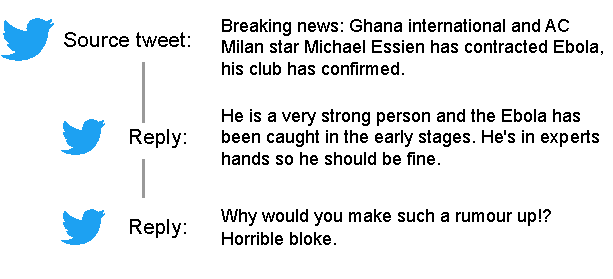
\includegraphics[scale=0.9]{obrazky-figures/pheme_essien.pdf}
    \caption{Example of fake breaking news from the PHEME dataset.}
    \label{fig:pheme_essien}
\end{figure}

In these cases, the help of content-based methods is crucial. Content-based methods rely only on the content of articles. They evaluate the linguistic and visual features from their input (e.g., style of writing, sensational headlines, etc.) and can operate using only the text of articles with no additional information needed.  The purpose of this thesis is to create a content-based classifier that relies only on text and uses it to compute the credibility of news articles and sources. The research goals can be defined as follows. (i) Understand how well can modern content-based approaches perform. (ii) Implement a method that interprets the results of the classifier to better understand what cues are exploited in the text. (iii) Use the classifier to determine the overall credibility of news publishers based on the articles they publish and compare the results with a state-of-the-art method. An interpretable classifier like this could be then used on downstream tasks, e.g., to improve available fact-checking systems by assigning a reliability score to the documents used as evidence. It could also be used to create a credibility ranking system for online sources that could even lead to creating a database of all internet publishers and their corresponding credibilities.

Chapter \ref{chap:definition} defines the problem of fake news detection and further explains the approaches and methods previously used by others in this field. Chapter \ref{datasets} presents a comprehensive review and analysis of publicly available datasets with fake news articles and discusses their suitability for this thesis. To train the classifier, only the NELA-2021 dataset is used in this thesis. The source-level labels in this dataset were expanded to all articles, meaning all articles received the label of the source that published them. This technique ensures a big dataset with lots of training data, however, as it is not guaranteed that all articles by an untrustworthy source are necessarily fake news, it may also bring some disadvantages. A similar technique of using source-level labels has been used by the authors of \cite{czech_paper}.

Chapter \ref{our-dataset} introduces the datasets created in this thesis and describes their preprocessing. Besides the NELA-GT-2021 dataset, another two datasets are used for testing purposes. The Merged dataset, created by merging three fake news datasets with article-level labels and the Fake News Interpretability (FNI) dataset, that was created by the author of this thesis and consists of 46 manually selected articles. The proposed methods for implementing the classifiers are described in chapter \ref{proposed-methods}. Chapter \ref{experiments} shows the evaluation results of the classifiers using multiple evaluation metrics.
Chapter \ref{chap:inter_anal} presents a qualitative analysis of the classifiers, including an interpretability analysis. In chapter \ref{chap:source_credibility} the implemented classifiers are applied to predict the reliability of media sources. Finally, chapter \ref{conclusion} provides a conclusion of this thesis together with suggestions for future work.




%%%%%%%%%%%%%%%%%%%%%%%%%%%%%%%%%%
% Previous work
\chapter{Fake News Detection}
\label{chap:definition}
This chapter provides a general introduction to the problem of fake news detection and the approaches used to implement it. The Cambridge Dictionary assigns fake news the following definition\footnote{\url{https://dictionary.cambridge.org/dictionary/english/fake-news}}.

\vspace{2mm}

\textbf{Definition 1:} Fake News --- False stories that appear to be news, spread on the internet or using other media, usually created to influence political views or as a joke.

\vspace{2mm}

Fake news is often used to manipulate and influence the opinions of readers during important events such as political elections. Other forms of fake news can be conspiracy theories or satire. 
In this thesis, a binary classifier model of fake news is created. The model expects the text of an article as its input and outputs the probability for two classes: reliable and unreliable. The output probabilities represent the credibility of the input article. The credibility of an article represents the extent to which the article can be perceived as trustworthy. The Cambridge Dictionary gives credibility the following definition\footnote{\url{https://dictionary.cambridge.org/dictionary/english/credibility}}.

\vspace{2mm}

\textbf{Definition 2:} Credibility --- The fact that someone can be believed or trusted.

\vspace{2mm}

Following is an overview of the methods previously used for fake news detection in this field. The methods could be classified into three categories based on the data they work with. They are content-based methods, knowledge-based methods and social context-based methods.
This thesis implements the approach of content-based methods. To base the decision, whether an article is reliable, solely on the style of its text is inherently not as reliable as using knowledge-based methods that verify the information written in the article against some database. There are, however, cases in which knowledge-based systems cannot be used, e.g., for recent news where none of the information written in the article can be verified. In these cases, a classifier based only on the stylistic features of text could be used complementary to a knowledge-based or a social context-based model.

\section{Content-based Methods}
For content-based methods, the actual content of the news is used to compute the credibility of the given article. These methods evaluate articles based on their linguistic or visual features. This means they extract lexical, semantic and syntactic characteristics capturing specific writing styles and sensational headlines that typically occur in fake news articles. 
Simple content-based methods often use the statistics of word occurrences in a corpus as the primary source of information. For these approaches, traditional methods like Term frequency-inverse document frequency (TF-IDF)\cite{tf-idf} can be used together with machine learning techniques, e.g., Decision trees, Support vector machines or Naive Bayes classifiers as in \cite{prev-work-dt} and~\cite{prev-work-bayes}.

Modelling the documents based only on word frequencies, however, limits the abilities of the classifiers. A much better approach is using word embeddings where the classifier knows not only the words that occur in a document but also has a sense of their meaning. These embeddings are usually represented as n-dimensional vectors trained to capture the relationships between words based on their co-occurrence in a document. The position of these vectors in this n-dimensional space then reflects their similarities. These embeddings can be created and trained directly from the text of documents using unsupervised methods like word2vec \cite{word2vec} and FastText \cite{fasttext}. It is also possible to obtain pre-trained word embeddings, e.g., the GloVe \cite{prev-work-glove} word representations.

These embeddings, however, do not exhibit the best performance because they employ fixed vectors for each word. This means that each word has only one vector representation that is the same in every context. A much better approach is using contextualized embeddings that enable multiple representations for a word based on the context of its surrounding words in the sentence. One example of a method that uses contextualized embeddings is the BERT \cite{bert} model.

The best results with content-based methods are generally achieved using deep neural networks. Using contextualized word embeddings and multiple layers of computation, they are able to exploit hidden features of documents and assess their credibility. Various neural network architectures are utilised for content-based methods.
Study \cite{prev-work-fndnet} proposed a deep convolutional neural network (FNDNet) for fake news detection. The authors used the GloVe pre-trained embeddings to create 100-dimensional word embeddings as the input for the network. The architecture consisted of 3 parallel convolutional layers whose results were concatenated together and run through several max pooling and dense layers. They used the Kaggle Fake News dataset, discussed in chapter \ref{datasets}, for training and evaluation and achieved an accuracy of 98.36\%. Achieving an accuracy of 98\% may look slightly suspicious. Therefore one of the objectives of this work is to create an interpretable classifier that would enable uncovering the biases that cause these exceedingly good results.

Authors of \cite{prev-work-dltechniques} implemented several fake news detection systems using 5 different classification techniques ---  Logistic regression (LR), Naïve Bayes (NB), Support vector machine (SVM), Random forest (RF) and a deep neural network (DNN) --- and compared their results. The experiments were performed on the LIAR dataset discussed later in this thesis in chapter \ref{datasets:liar}. The results showed that the DNN classifier outperformed the other traditional machine learning methods as it achieved an accuracy of 91\% followed by the NB method which achieved an accuracy of 89\%.

In both of the mentioned methods, the models were trained using pairs of text and a label that represents its credibility. A different approach was chosen by the authors of \cite{bert-exbake}. Their approach tried to detect fake news by classifying the stance of the text in the body of an article relative to its headline. The body can either agree, disagree, discuss or be unrelated to the headline resulting in 4 different class labels. To train the model they used the FNC-1\footnote{\url{https://github.com/FakeNewsChallenge/fnc-1}} dataset.
The training set consisted of a total of 2587 pairs of headline and body texts and the class label for each pair. The authors used the BERT model with its pre-trained embeddings and fine-tuned the model by classifying the data using linear and softmax layers into the four classes. Weighted cross-entropy was used as the loss function because of a big imbalance in the class labels. The classifier achieved an F1 score of 0.74.


\section{Knowledge-based Methods}
On the other hand, knowledge-based methods use external sources to check the veracity of claims extracted from the articles. This process is also known as automated fact-checking and usually consists of three stages as described in \cite{prev-work-fact-checking}: (i) claim detection to identify claims that require verification; (ii) evidence retrieval to find sources supporting or refuting the claims; (iii) claim verification to assess the veracity of the claim based on the retrieved evidence.

In other words, automated fact-checking creates evidence-grounded systems which for a given claim identify relevant sources and then use these sources to predict the veracity of the given claim.\cite{claim-dissector}.
The authors of \cite{fever} introduced a new dataset suitable for verification against textual sources called FEVER (Fact Extraction and VERification). This dataset is further described in section \ref{datasets:fever}. Other widely used datasets include FaVIQ \cite{faviq} and REALFC \cite{realfc}. Most state-of-the-art systems are based on a 3-stage approach as described in \cite{claim-dissector}: for a claim, they retrieve relevant documents, rank parts of these documents based on their relevance and predict the veracity of the given claim from the top-K ranked parts.
Another approach was introduced by the authors of \cite{claim-dissector}. They created a latent variable model called Claim-Dissector. This model combines the ranks of top-relevant, top-supporting and top-refuting provenances\footnote{Parts of the text, sentences, paragraphs, etc.} and predicts the veracity of a claim as the linear combination of its per-provenance probabilities.

\section{Social Context-based Methods}
Social context-based methods are often applied to social media as they incorporate features from user profiles to the fake news detection problem. They often use previous interactions of users and model their tendency to share information from doubtful sources. The datasets used by these methods are often collected from social media networks like Twitter or Facebook. One of these datasets is the PHEME dataset described in section \ref{datasets:pheme}. It consists of a collection of rumours and non-rumours posted during breaking news on Twitter. Besides the tweets, the dataset also contains additional information about users — their time zones, locations, number of followers, profile pictures, etc.

Social context methods usually aim to extract information by analysing the connectivity of users and articles. To do this they often use Bayesian probability graphical models as in \cite{unsupervised_graph}, or various types of matrix and tensor factorization \cite{tensor_paper}, \cite{trifn}. 

Matrix factorization is a technique commonly used also among recommender systems. In this case, the matrix composes of interactions between users (rows of the matrix) and articles (columns of the matrix). The actual values inside the matrix can be the number of interactions, minutes spent reading, a rating, etc. The interaction matrix is then decomposed as the product of two or three matrices such that it maps both users and articles to a joint latent factor space where the interactions are modelled as the inner product in that space. Examples of these models include LDA \cite{lda} and SVD \cite{svd}.
For fake news detection, a similar approach can be used. The interaction matrix is decomposed into a matrix of user and article features. New interactions can be modelled as the product of a user-feature vector and an article-feature vector resulting in a probability of this user sharing the article. 

Authors of \cite{tensor_paper} proposed a semisupervised approach for classifying fake news posts that combines tensor factorization and classification in a joint learning process. The interactions of users with posts and users with other users are modelled in a 3rd-order tensor. To decompose this tensor they employ the Canonical/Parafac (CP) factorization \cite{parafac} using a least-squares loss. The tensor is decomposed into three matrices A, B, and C, where A represents the posts-factor matrix, and B and C represent the users-factor matrices. To capture the class information of posts a classification error term is added to matrix A.

Authors of \cite{trifn} described the process of fake news dissemination on social media as a tri-relationship --- the relationship among publishers, news pieces, and users. They created an embedding model called TriFN, which models these relationships simultaneously for fake news detection.
It consists of five major components: a news contents embedding component, a user embedding component, a user-news interaction embedding component, a publisher-news relation embedding component, and a semi-supervised classification component
The news contents embedding component is a bag-of-words feature matrix. The user embedding component is constructed as a user-user adjacency matrix, that represents friendships among users. The user-news component is a matrix that states which users shared which news articles, similar to the publisher-news component that models which articles were published by which publishers. The semi-supervised classification component learns to predict unlabeled news articles. The components then employ various factorization approaches, e.g., nonnegative matrix factorization, to create feature vectors that are then used in the TriFN embedding. 

Social context-based methods are often used in combination with content-based approaches to utilize their best abilities and further improve fake news detection. Authors of \cite{hybrid} created a hybrid model based on integrating a graph neural network on the propagation of news and bi-directional encoder representations from the transformers model on news content. 

\section{Methods for Source Credibility}
This thesis studies predicting the credibility of both articles and the media sources that publish them. The credibility of sources has also been researched in previous work. In \cite{source-reputation}, the authors created an interpretable joint graphical model for fact-checking from crowds which uses claims, headlines and sources. Each claim has an assigned veracity (correctness) that can be true, false or unknown. Each headline corresponds to a source and has a stance towards the claim. The stance can be for, against or merely observing the claim. To predict the veracity of claims the authors defined a multiclass logistic regression model parameterized by R (the reputation of a source), that uses all source stances for the claim as features. In this scheme, the reputation of source R is a parameter learned by the model.

Another approach was applied by the authors of \cite{declare} who created a neural network model called DeClarE that predicts the credibility of claims by aggregating signals from external evidence articles, the language of these articles and the trustworthiness of their sources. To predict the credibility of a claim the architecture combines the article and claim embeddings to get the claim-specific attention weights. The article embeddings are run through bidirectional LSTM to create article representations. These representations are combined with the attention weights and concatenated with the claim-source embeddings and the article-source embeddings. This is then passed through several dense layers and softmax to predict the credibility of the claim. After training the model, the authors analysed the learned article-source and claim-source embeddings using PCA to project the representations. They found that fake news sources were separated from mainstream media and sources with similar opinions were located close to each other in the embedding space.

The methods of predicting the credibility of sources implemented in this thesis are compared with another method which uses the citations between sources to assess their credibility. This method is briefly explained in chapter \ref{chap:source_credibility}.



%%%%%%%%%%%%%%%%%%%%%%%%%%%%%%%%%%
% Analysis of available datasets
\chapter{Fake News Datasets}
\label{datasets}
An extensive part of this thesis was to create a review of available fake news datasets. Choosing the right dataset is crucial for training a model that generalizes as much as possible, without focusing on irrelevant biases, as explained in \cite{debias}. It was first necessary to define the requirements of our system. The chosen dataset should consist of news articles and contain the following fields: (i) the text of the article; (ii) a binary label identifying whether the article is true or fake; (iii) optionally also the name of the source that published the article. This section provides a thorough analysis of several publicly available datasets. Each dataset was evaluated for its suitability for this thesis.

Table \ref{tab:datasets_comp} shows a comparison of the studied datasets. For training the models, the NELA-GT-2021 dataset was used in this thesis. Apart from NELA, other datasets were used. The Fake news dataset, Fake or real news dataset and FakeNewsNet were merged and used for further testing of the created models. The following sections discuss the datasets in further detail.

\begin{table}[H]
    \centering
\begin{tabular}{c|c|c|c|c|}
\textbf{Dataset} & \cellcolor[HTML]{FFFFFF}\textbf{Type} & \textbf{Size} & \cellcolor[HTML]{FFFFFF}\textbf{Labels} & \textbf{Sources} \\ \hline
Fake News          & news articles & 20,800      & 2  & No  \\
Fake or Real News  & news articles & 6,335       & 2  & No  \\
NELA-GT-2021       & news articles & 1,8 million & 3* & Yes \\
FakeNewsNet        & news articles & 422         & 2  & Yes \\
Liar               & statements    & 2,836       & 6  & -   \\
FEVER              & statements    & 185,445     & 3  & -   \\
PHEME              & tweets        & 6,425       & 2  & -   
\end{tabular}    
    \caption{Comparison of the examined datasets. *The labels in the NELA dataset are on a source level (label per source, not per each article).}
    \label{tab:datasets_comp}
\end{table}


\section{Fake News Dataset}
\label{fake_news_dataset}
The first reviewed dataset is called the Fake news dataset. It was published in 2018 and is available on the Kaggle website\footnote{\url{https://www.kaggle.com/competitions/fake-news/data}}. There is no specific information available on how this dataset was collected. The author only stated that it was created by merging several fake news datasets available on Kaggle and that he would not vouch for its quality in general as it may contain lots of artefacts that limit its usefulness in training a more generalizable model. Despite this knowledge. the dataset was used in some publications, including \cite{prev-work-fndnet}. Table \ref{tab:fake_news_table} shows the fields in the training dataset.

% \begin{itemize}
%     \item id = unique id for a news article
%     \item title = the title of the article
%     \item author = author of the article
%     \item text = text of the article; could be incomplete
%     \item label = binary label that marks the article as potentially unreliable (1-unreliable, 0-reliable)
% \end{itemize}

\begin{table}[H]
    \centering
\begin{tabular}{c|c|l}
\rowcolor[HTML]{FFFFFF} 
\textbf{Column} & \textbf{Type}                  & \textbf{Description}                \\ \hline
title           & text                           & Headline of the article             \\
author          & text                           & Author of the article               \\
text            & text                           & The text in the body of the article \\
label & integer & \begin{tabular}[c]{@{}l@{}}Binary label that marks the article as potentially unreliable \\ (1---unreliable, 0---reliable)\end{tabular}
\end{tabular}
    \caption{Fields inside the Fake News Dataset.}
    \label{tab:fake_news_table}
\end{table}

The test dataset contains the same fields except for the labels, as the results were meant to be submitted to the authors for evaluation. One drawback of this dataset is that the articles contain no sources. The only available information is the name of the author, which is not a useful feature with respect to the aims of this thesis.

The training dataset contains 20,800 articles and the test dataset 5,200 articles. The distribution of reliable and unreliable articles is well-balanced. The articles contain on average 773 words. The topic of the articles is not specified. After analysing the most used words it can be assumed that most articles revolve around politics, most probably in the U.S. as the most common words were Donald Trump, Hillary Clinton, America and the United States.


\section{Fake or Real News Dataset}
\label{fake_or_real_news}
Fake or real news is a small dataset presented in \cite{fake_or_real_dataset} as part of their survey on fake news prediction. It is available on Kaggle.com\footnote{\url{https://www.kaggle.com/datasets/rchitic17/real-or-fake}}. The dataset consists of 6,335 news articles. Each article is assigned a binary label identifying it as either real or fake. The distribution of labels is well-balanced with approximately half of the articles being real and the other half fake. The dataset contains the following fields.


\begin{table}[H]
\centering
    \begin{tabular}{c|c|c}
    \textbf{Column} & \cellcolor[HTML]{FFFFFF}\textbf{Type} & \cellcolor[HTML]{FFFFFF}\textbf{Description} \\ \hline
    title & text & Headline of the article             \\
    text  & text & The text in the body of the article \\
    label & text & Binary label (REAL/FAKE)           
    \end{tabular}
    \label{tab:fake_or_real_fields}
    \caption{Fields for each article in the Fake or real news dataset.}
\end{table}


In some cases, the text contains the name of the author or media source that published the article. However, for most articles, this information is unknown. The topics of the articles are also not known.


\section{NELA-GT-2021}
\label{nela}
This section discusses the NELA-GT-2021 dataset\footnote{\url{https://dataverse.harvard.edu/dataset.xhtml?persistentId=doi:10.7910/DVN/RBKVBM}}. The 2021 version of the NELA-GT dataset is the fourth publication of this dataset and is further described by the authors in~\cite{nela-paper}. 
The dataset was created by scraping the content of web articles from news sources on the internet published in 2021. It consists of approximately 1.8 million articles from 348 different sources. The scraped articles contain the following fields.

\begin{table}[H]
    \centering
\begin{tabular}{c|c|l}
\rowcolor[HTML]{FFFFFF} 
\textbf{Column} & \textbf{Type}               & \textbf{Description}                              \\ \hline
id              & text (primary key)          & Identifier of the article                         \\
date            & text                        & Publication date string in yyyy-mm-dd format      \\
source          & text                        & Name of the source that published the article     \\
title           & text                        & Headline of the article                           \\
content         & text                        & The text in the body of the article               \\
author          & text                        & Author of the article (may be empty)              \\
published       & text                        & Publication date string as provided by the source \\
published\_utc  & integer                     & Publication time as unix time stamp               \\
collection\_utc & integer                     & Collection time as unix time stamp                \\
url             & text                        & URL of the article                               
\end{tabular}
    \caption{Structure of data collected for an article in the NELA-GT-2021 dataset.}
    \label{tab:nela_fields}
\end{table}

An important part of the dataset, besides the actual content of the scrapped articles, is a categorization of the collected news sources. In a separate file, called labels.csv, there is a label for each source defining its reliability. The label can have one of the following values.

\begin{itemize}
    \item 0 --- marks the given source as reliable
    \item 1 --- marks the given source as unreliable
    \item 2 --- marks the given source as mixed
\end{itemize}

To create these source-level labels, the authors of the dataset used a website specialized in rating news sources on the internet called Media Bias / Fact Check (MBFC)\footnote{\url{https://mediabiasfactcheck.com/}}. This website contains an extensive database of more than 5400 media sources and journalists, categorized by two main criteria: bias and factuality. 
The \emph{bias of a news source defines a prejudice or an inclination in favour of or against one thing, person or group}. The MBFC website recognizes the following types of bias:

\begin{itemize}
    \item Least Biased --- Most credible media sources that have minimal bias, factual reporting and are usually well sourced.
    
    \item Left Bias ---  Moderately to strongly biased toward liberal causes through story selection and/or political affiliation. These sources may be misleading and untrustworthy.
    
    \item Left-Center Bias --- Slight to moderate liberal bias, usually trustworthy sources.

    \item Right Bias --- Moderately to strongly biased toward conservative causes through story selection and/or political affiliation. These sources may be misleading and untrustworthy.

    \item Right-Center Bias --- Slight to moderate conservative bias, generally trustworthy.

    \item Conspiracy-Pseudoscience --- These sources publish unverifiable information that is usually not supported by evidence, may be untrustworthy.

    \item Questionable Sources --- Extreme bias, promotion of propaganda and conspiracies, no sourcing of credible information and fake news. These sources are very untrustworthy.

    \item Pro-Science --- These sources publish evidence-based information through the use of credible scientific sourcing. Unbiased and trustworthy.

    \item Satire --- These sources use humour, irony, exaggeration, or ridicule to expose and criticize people or other topics. They usually claim to be satirical and do not try to deceive.
\end{itemize}

The bias of media sources may help to identify not only the inclination towards specific topics but also the credibility of published articles. The MBFC website recognises two main biases of untrustworthy sources: Conspiracy-Pseudoscience and Questionable Sources, with the latter being marked as likely very untrustworthy. On the other hand, sources marked as Pro-science or Least Biased can be generally considered credible. 
Another measure that the MBFC website uses to classify media sources is the factuality score. \emph{Factuality represents how much the reporting of a source resolves around actual well-sourced facts that can be proven}. It may hold one of the following six values:

\begin{multicols}{2}
\begin{itemize}
    \item Very Low
    \item Low
    \item Mixed
    \item Mostly Factual
    \item High
    \item Very High
\end{itemize}
\end{multicols}

A source with a very low or low factuality could be considered untrustworthy, whereas sources with very high or high factualities are likely to publish credible information. The final labels of a given media source in the NELA-GT-2021 dataset are constructed as follows: \cite{nela-paper}

\begin{itemize}
    \item 0 (reliable) --- sources with high or very high factuality
    \item 1 (unreliable) --- sources with Conspiracy-Pseudoscience bias or very low / low factuality
    \item 2 (mixed) --- sources with mixed factuality
\end{itemize}

The distribution of source labels in the dataset can be seen in figure \ref{fig:labels_all_dist}. As the figure shows, the distribution of media sources among labels is not very even. The number of unreliable sources is more than double the number of reliable and more than four times the number of sources marked with the mixed label. This proportion changes when looking at the total number of articles for each label. \emph{There are more unreliable sources but more reliable articles in the dataset}. In total, the dataset contains 603,894 articles from reliable sources, 490,345 articles from unreliable sources and 416,673 articles from mixed sources as shown in figure \ref{fig:articles_per_label}.

\begin{figure}[H]
\centering
\begin{subfigure}{.5\textwidth}
  \centering
  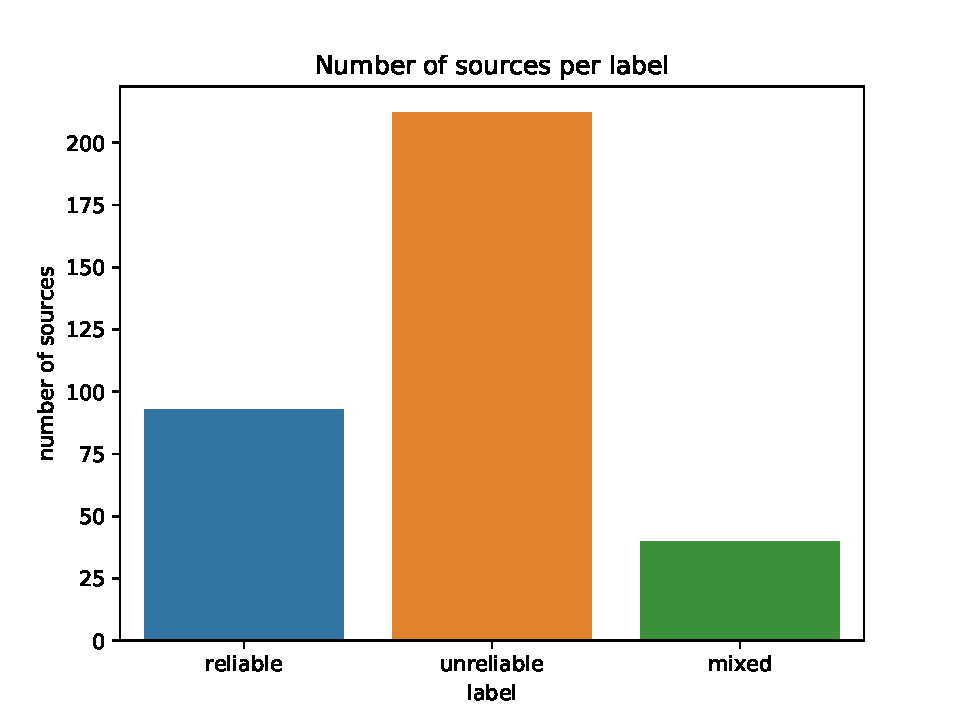
\includegraphics[width=\linewidth]{obrazky-figures/labels_all_dist.pdf}
  \caption{The number of sources per label.}
  \label{fig:labels_all_dist}
\end{subfigure}%
\begin{subfigure}{.5\textwidth}
  \centering
  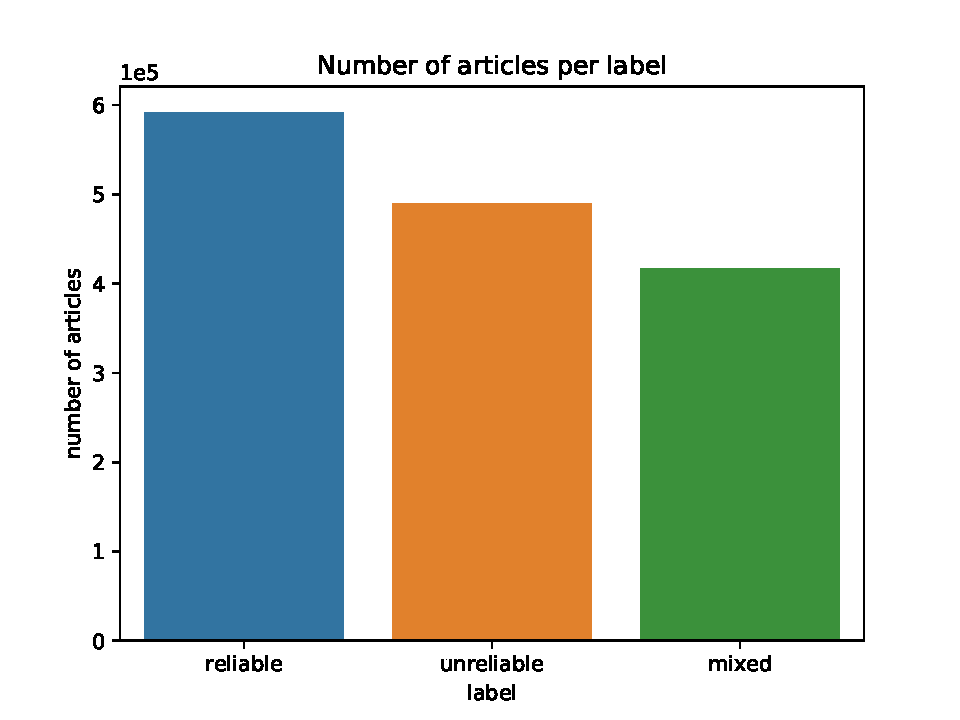
\includegraphics[width=\linewidth]{obrazky-figures/articles_per_label.pdf}
  \caption{The number of articles per label.}
  \label{fig:articles_per_label}
\end{subfigure}
\caption{Distribution of labels in the NELA-GT-2021 dataset.}
\label{fig:test}
\end{figure}

Due to the imbalance in the distribution of labels, it is obvious that the most frequent types of bias are the ones that imply untrustworthy sources. Indeed the most common bias in the dataset is Conspiracy-Pseudoscience, followed by the Questionable Source and Left-Center bias. The number of sources per bias is shown in figure \ref{fig:bias_dist}.
It is also interesting to see what are the most common biases in each label group. As already mentioned earlier, sources labelled as unreliable are those with Conspiracy-Pseudoscience bias or low/very low factuality. It is therefore straightforward that the most common biases among unreliable sources are Conspirtacy-Pseudoscience (159 sources), Questionable-Source (52 sources) and one source with Right bias. 
Reliable sources, on the other hand, contain sources from 6 different biases: Left-Center (40 sources), Left (18 sources), Center (13 sources), Right-Center (12 sources), Pro-Science (6 sources), Right (4 sources). 
Sources with the Mixed label are also spread between several biases: Right (17 sources), Left-Center (11 sources), Left (11 sources) and Right-Center (1 source). The number of sources per bias in each label can be also seen in figure \ref{fig:bias_by_src}

\begin{figure}[H]
    \centering
    \begin{subfigure}{.5\textwidth}
      \centering
      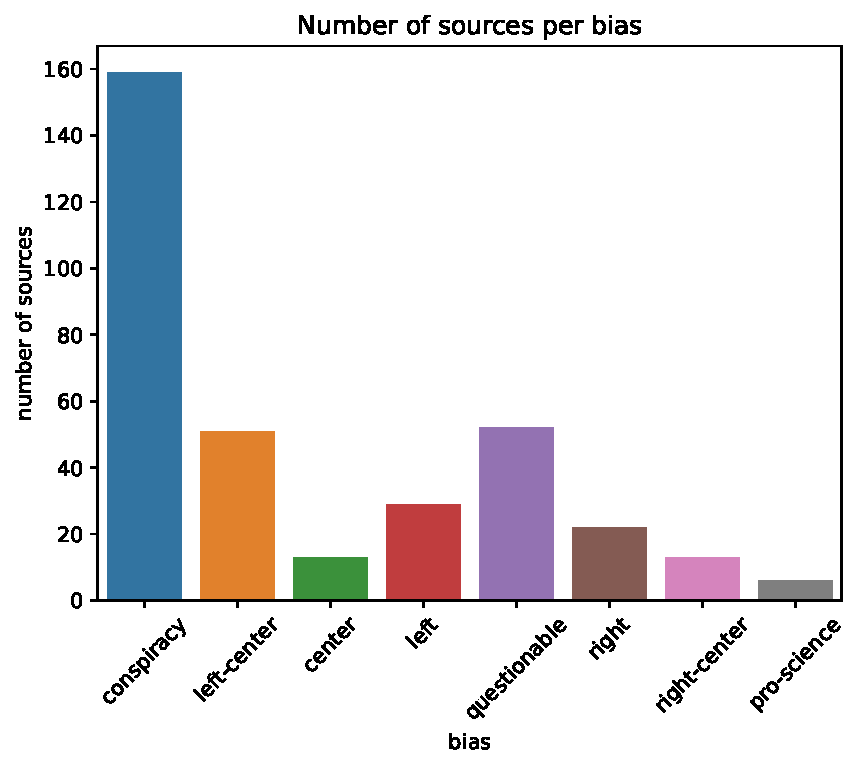
\includegraphics[width=\linewidth]{obrazky-figures/bias_dist.pdf}
      \caption{Number of sources per bias.}
      \label{fig:bias_dist}
    \end{subfigure}%
    \begin{subfigure}{.5\textwidth}
      \centering
      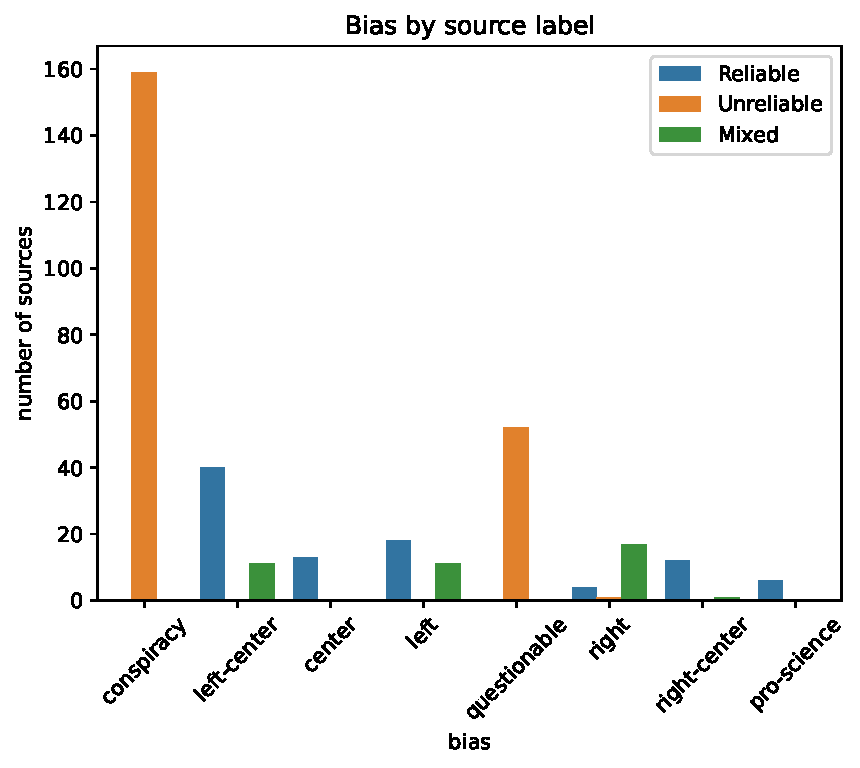
\includegraphics[width=\linewidth]{obrazky-figures/bias_by_src.pdf}
      \caption{Number of sources per bias for each label.}
      \label{fig:bias_by_src}
    \end{subfigure}
    \caption{Analysis of the sources and their bias in the NELA-GT-2021 dataset.}
    \label{fig:test2}
\end{figure}

Similarly, we can have a look at the number of sources per factuality score. This can be seen in figure \ref{fig:factuality_dist}. Figure \ref{fig:factuality_by_src} then shows the number of sources per factuality for each label. It is evident that sources labelled as unreliable generally possess lower factuality scores. Interestingly, there is one source with mixed factuality marked as reliable (Daily Telegraph - UK). 

\begin{figure}[H]
    \centering
    \begin{subfigure}{.5\textwidth}
      \centering
      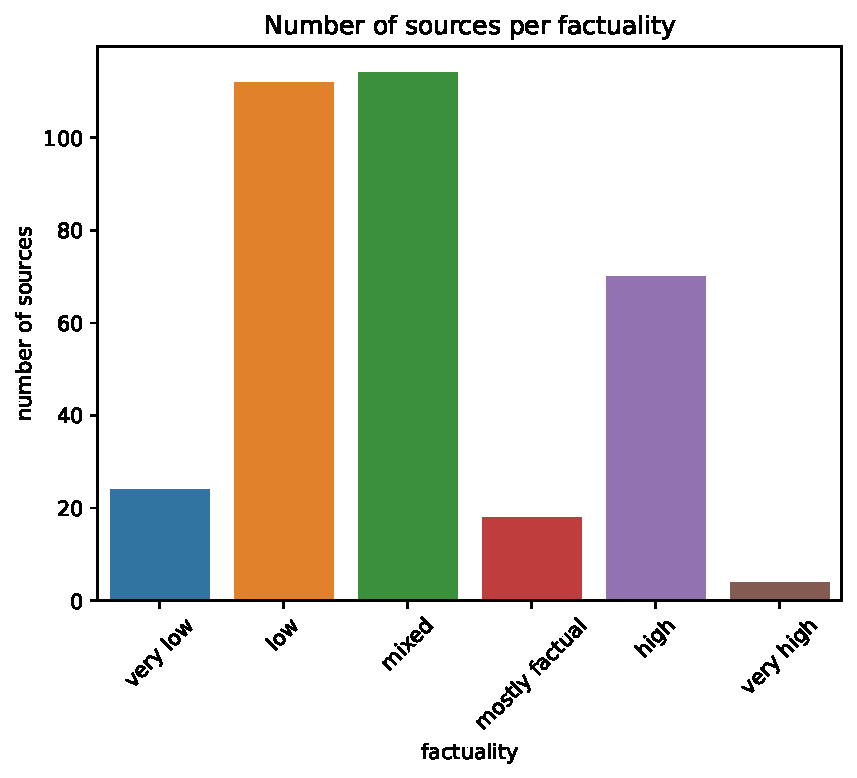
\includegraphics[width=\linewidth]{obrazky-figures/factuality_dist.pdf}
      \caption{Number of sources per factuality score.}
      \label{fig:factuality_dist}
    \end{subfigure}%
    \begin{subfigure}{.5\textwidth}
      \centering
      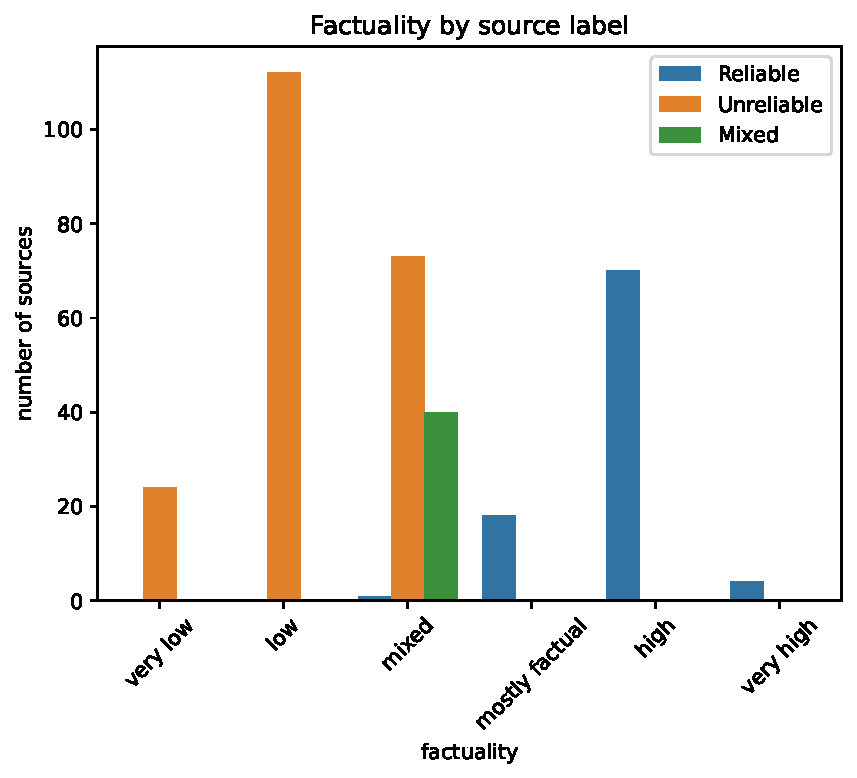
\includegraphics[width=\linewidth]{obrazky-figures/factuality_by_src.pdf}
      \caption{Number of sources per factuality for each label.}
      \label{fig:factuality_by_src}
    \end{subfigure}
    \caption{Analysis of the sources and their factuality score in the NELA-GT-2021 dataset.}
    \label{fig:test3}
\end{figure}

The actual content of articles in the NELA dataset had to be slightly modified as some of the texts in the dataset are copyrighted. For articles with more than 200 tokens, 7 consecutive tokens are replaced with an at symbol ‘@’ every 100 tokens. For articles with fewer than 200 tokens, only 5 tokens are replaced with ‘@’ every 20 tokens. This transformation polishes the articles to make them useless for anyone who would want to use the dataset to consume news while still keeping most of the content useful for analysis. Features like the relative frequency of words are not affected by this transformation as it occurs with no regard to context. Following is an example of the polished text in the dataset:

\begin{center}
    \texttt{The proposals are primarily in response to President Joe Biden ’ s @ @ @ @ @ @ @ least 100 employees to get vaccinated or tested regularly. Randy Zook , president of the state Chamber of Commerce , warned lawmakers that the proposal could force employers between choosing whether to violate state law or federal regulations.}
\end{center}

The NELA-GT-2021 dataset was found suitable for this thesis. It is a large dataset with source-level labels and besides the content of articles, it contains additional information about where and when they were published. Polishing the text with special symbols should have no effect on the analysis. More details about how this dataset is used in this thesis can be found in chapter \ref{our-dataset}.


\section{FakeNewsNet}
\label{fake_news_net}
FakeNewsNet is a dataset available at Kaggle.com\footnote{\url{https://www.kaggle.com/code/sohamohajeri/buzzfeed-news-analysis-and-classification/data}}. It consists of 422 news articles collected by Buzzfeed\footnote{\url{https://www.buzzfeed.com/}} and Politifact\footnote{\url{https://www.politifact.com/}}. Each article is assigned a binary label indicating whether the article is real or fake. Besides labels, this dataset contains additional information, some of which is displayed in table \ref{tab:fakenewsnet}.


\begin{table}[H]
    \centering
    \begin{tabular}{c|c|l}
    \textbf{Column} & \cellcolor[HTML]{FFFFFF}\textbf{Type} & \cellcolor[HTML]{FFFFFF}\textbf{Description} \\ \hline
    title        & text & Headline of the article             \\
    text         & text & The text in the body of the article \\
    url          & text & Url of the article                  \\
    authors      & text & Names of authors of the article     \\
    source       & text & Source that published the article   \\
    publish date & text & Publication date of the article     \\
    movies       & text & Urls to all videos in the article   \\
    images       & text & Urls of all images in the article  
    \end{tabular}
    \caption{Fields in the FakeNewsNet dataset.}
    \label{tab:fakenewsnet}
\end{table}

The distribution of labels is very well-balanced with half of the articles being fake and the other half real. This dataset is a great candidate for the purposes of this thesis. It consists of news articles and contains both labels and sources. However, due to its size of only 422 articles, it may not be enough to train a robust classifier and it is therefore only used for testing.


\section{Liar Dataset}
\label{datasets:liar}
Introduced in \cite{liar}, the Liar dataset consists of 12,836 statements collected in various contexts from politifact.com. Each statement was manually assigned a label evaluating it for its truthfulness. The dataset considers six fine-grained labels, in order from less to most trustworthy: pants-fire, false, barely-true, half-true, mostly-true, and true. The average length of a statement in the dataset is 18 words.
The statements in the dataset are categorized into 4,535 different subjects. The most common ones are health care, taxes, education, elections and immigration. Each statement also specifies the speaker, meaning the person responsible for the statement. The most common speakers in the dataset are Barack Obama, Donald Trump, Hillary Clinton and Mitt Romney. Table \ref{tab:liar_columns} shows all fields in the Liar dataset.
\begin{table}[h]
    \centering
    \begin{tabular}{c|c|l}
    \textbf{Column} & \cellcolor[HTML]{FFFFFF}\textbf{Type} & \cellcolor[HTML]{FFFFFF}\textbf{Description}  \\ \hline
    label       & text    & Label of the statement                  \\
    statement   & text    & Content of the evaluated statement      \\
    subject     & text    & The topic/subject of the statement      \\
    speaker     & text    & Name of the speaker                     \\
    speaker job & text    & Job title of the speaker                \\
    state       & text    & State which the speaker is representing \\
    party       & text    & Party affiliation of the speaker        \\
    barely-true & integer & Barely-true counts                      \\
    false       & integer & False counts                            \\
    half-true   & integer & Half-true counts                        \\
    mostly-true & integer & Mostly-true counts                      \\
    pants-fire  & integer & Pants on fire counts                    \\
    venue           & text                                  & The venue/location of the speech or statement
    \end{tabular}
    \caption{Structure of data in the Liar dataset.}
    \label{tab:liar_columns}
\end{table}
The barely-true, false, half-true, mostly-true, and pants-fire fields in the dataset, represent the total number of statements by the speaker that were assigned the given label. Figure \ref{fig:liar_labels} shows the number of statements for each label. The distribution of labels is well-balanced except for the pants-fire label. 
\begin{figure}[h]
    \centering
    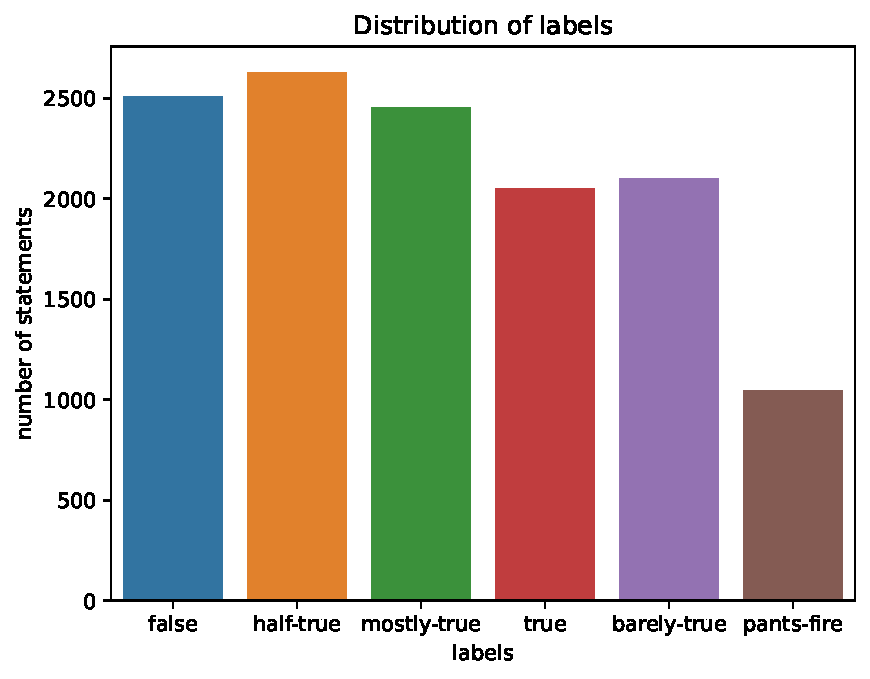
\includegraphics[scale=0.6]{obrazky-figures/liar_labels.pdf}
    \caption{Number of statements by label in the Liar dataset.}
    \label{fig:liar_labels}
\end{figure}

The Liar dataset is one of the most used datasets for fake news detection. Its manually assigned labels guarantee a big level of authenticity. However, as the dataset only contains short statements, it is not suitable for training a classifier working with entire news articles. Therefore, it was not found suitable for the purpose of this thesis.


\section{FEVER}
\label{datasets:fever}
FEVER, which stands for Fact Extraction and Verification, is a dataset for verification against textual sources introduced in \cite{fever}. The dataset consists of 185,445 claims generated by altering sentences extracted from Wikipedia. For each claim, there is evidence that can be used to verify it. The claims are labelled as Supports, Refutes or Not enough info indicating whether the evidence supports or refutes the claim. On average, a claim contains only 8 words. Some examples of claims from the FEVER dataset are:

\begin{center}
    \texttt{Roman Atwood is a content creator.} \\
    \texttt{Charles Woodruff Yost died.} \\
    \texttt{Portugal leads the European Union.} \\
    \texttt{Muhammad Ali was a model of racial pride for resistance to white domination.}
\end{center}

\begin{table}[H]
    \centering
    \begin{tabular}{c|c|l}
    \textbf{Column} & \cellcolor[HTML]{FFFFFF}\textbf{Type} & \cellcolor[HTML]{FFFFFF}\textbf{Description} \\ \hline
    verifiable & text & Specifies whether given claim is verifiable or unverifiable  \\
    label      & text & Specifies whether the evidence refutes or supports the claim \\
    claim      & text & The evaluated claim                                          \\
    evidence   & text & Reference to the evidence refuting or supporting the claim  
    \end{tabular}
    \caption{Structure of data in the FEVER dataset.}
    \label{tab:fever_columns}
\end{table}

Table \ref{tab:fever_columns} shows the contents of the FEVER dataset. Figure \ref{fig:fever_labels} shows the distribution of labels in the dataset. It may be seen that the majority of claims are supported by the evidence as the number of claims in this class is more than double the number of claims that are refuted. 

\begin{figure}[H]
    \centering
    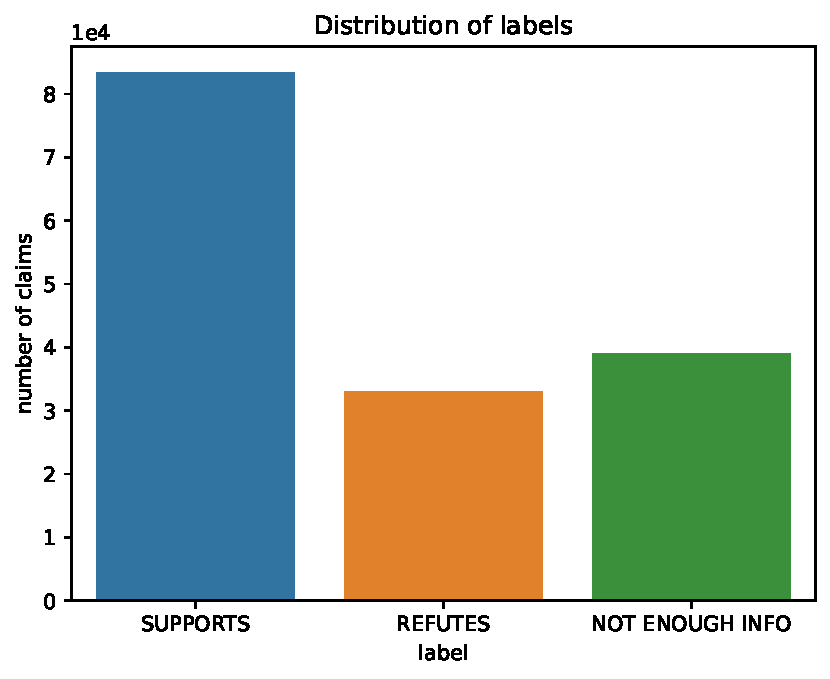
\includegraphics[scale=0.6]{obrazky-figures/fever_labels.pdf}
    \caption{Number of claims by label in the FEVER dataset.}
    \label{fig:fever_labels}
\end{figure}

The main use of the FEVER dataset is for fact-checking and extraction tasks. It could, however, also be used for fake news detection tasks as the labels that indicate whether the evidence supports or refutes the claim, could also be interpreted as whether the claim is true or fake. This interpretation would enable the training of a classifier. However, given the short nature of given claims, it is not suitable for classifying long texts of news articles.



\section{PHEME}
\label{datasets:pheme}
PHEME was introduced in \cite{pheme}. It is a dataset containing a collection of rumours and non-rumours posted during breaking news related to 9 different events on Twitter. Besides the tweets, the dataset also contains information about the authors of the tweets, their locations, number of followers, links to their profiles etc. The dataset also contains all the reactions to the posted rumours/non-rumours tweets including comments and likes. 
In total, there are 4,023 non-rumour and 2,402 rumour tweets. This dataset is ideal for use in social context-based methods where the classifier evaluates the interactions of users. It is, therefore, not suitable for this thesis.



%%%%%%%%%%%%%%%%%%%%%%%%%%%%%%%%%%
% Analysis of the test dataset
\chapter{Creating Datasets For This Thesis}
\label{our-dataset}
The previous chapter analyzed available fake news datasets. This chapter presents the final datasets that are used for training and testing the classifiers in this thesis. In total, three different datasets are used. The dataset used for training is a preprocessed form of the NELA-GT-2021 dataset. The other two datasets are used only for testing. These datasets are the Merged dataset --- created by merging three different fake news datasets --- and the Fake News Interpretability dataset ---  created especially for this thesis by manually collecting several fake and real articles.




\section{NELA Dataset}
\label{nela-my}
The dataset used for training the classifiers in this thesis was created by modifying the NELA-GT-2021 dataset. This section describes the preprocessing of this dataset as displayed in figure \ref{fig:nela_prepproc}. The first step was expanding the source-level labels to all articles. This means that all articles were assigned the label of their source. After expanding the labels, all articles labelled as mixed were removed. Only the articles published by reliable and unreliable sources were kept in the dataset. The reason for removing mixed labels is that the articles published by mixed sources may contain both reliable and unreliable articles, making it harder for the classifier to correctly learn to detect fake news. 
% The experiments performed on a classifier trained with mixed labels showed a significant degradation in the performance and it is further discussed in chapter \ref{experiments}. 

The next preprocessing step was keyword filtering. After initial manual analysis, it was found that the text often contains simple cues, e.g., source name, author name, etc., which could be leveraged by the model without analyzing the semantics of the language. To investigate the exploitation of the easy cues by the models, an analysis using the baseline model was performed. The baseline model, described in chapter \ref{baseline}, uses a Multinomial Naive Bayes (MNB) classifier and TF-IDF.
% As a consequence of extending the labels of sources to all their articles, there is a possibility that the created classifiers would actually learn to classify sources instead of labels. The classifier could, for example, learn that all articles published by CBS can be considered reliable and would therefore learn to identify keywords, e.g.,, the name of the source. 

\begin{figure}[H]
    \centering
    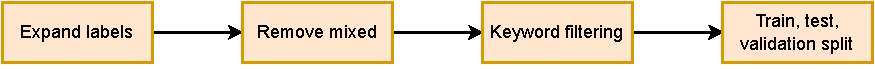
\includegraphics[scale=1]{obrazky-figures/nela_preproc.pdf}
    \caption{Preprocessing steps of the NELA dataset.}
    \label{fig:nela_prepproc}
\end{figure}

In the training process, the MNB classifier learns the probabilities of all words for each class. This means each word in the dataset is assigned a probability for classes \texttt{reliable} and \texttt{unreliable}. It is then possible to look at the words with the highest probabilities for each class and hence display the words that contribute the most to the decision of the classifier. The importance of word $x$ is computed as follows.

\begin{equation}
    \operatorname{Imp}(x) = \displaystyle{\frac{P (x | reliable)} {P (x | unreliable)}}
    \label{eq:imp}
\end{equation}
where $P (x | reliable)$ is the probability of $x$ for class \texttt{reliable} and $P (x | unreliable)$ is the probability of $x$ for class \texttt{unreliable}. Words with high values are more important to the \texttt{reliable} class and vice versa. The filtering was performed by comparing each word from the articles with a defined set of keywords. If a word matches one of the defined keywords it is removed from the text. The filtering was performed in two iterations with each iteration having its own set of keywords. The following keywords were used in the iterations.

\begin{itemize}
    \item Iteration 1 --- (395 keywords) filtering names of sources in various forms as they appear in the dataset (e.g., \texttt{cbs}, \texttt{cbsn}, \texttt{upi}, \texttt{ipolitics}, \texttt{foxnews}, \texttt{tass}, etc.).
    \item Iteration 2 --- (19 keywords) filtering source-specific terms discovered during the analysis of the most important words for each class. This includes football-related terms --- as the sources writing about football are considered reliable, the classifier learned to interpret football-related terms as a sign of reliability (especially names of players, coaches and football clubs). Other source-specific keywords include, e.g., \texttt{garda}, \texttt{gardaí} (names of the police department in Ireland used by a reliable source The Irish Times), \texttt{quijano} (name of a cbs news reporter Elaine Quijano), \texttt{paypal}, and currency abbreviations (heavily used by an unreliable source --- Infinite Unknown --- at the end of their articles where they ask readers for donations).
\end{itemize}

Table \ref{tab:kw_filtering} shows the most important words for each class in the original dataset and after keyword filtering. It can be seen that in the original dataset, there are a lot of source names among the most important words (e.g., \texttt{cbsn}, \texttt{upi}, \texttt{ipolitics}, \texttt{nrplus}, \texttt{sitsshow}, \texttt{lifesitenews}). After removing them in the first iteration, the 20 most important words, discovered with the method in equation \ref{eq:imp}, were manually analysed. Multiple source-specific terms were identified, e.g., \texttt{gardaí}, \texttt{arteta} --- the coach of Arsenal football club, currency abbreviations, etc. Therefore the second iteration was applied to remove these terms.


\begin{table}[H]
    \centering
\begin{tabular}{c|c|c|c|c|c}
\multicolumn{2}{c|}{\textbf{Original}}                        & \multicolumn{2}{c|}{\textbf{Iteration 1}}   & \multicolumn{2}{c}{\textbf{Iteration 2}}   \\ \hline
\multicolumn{1}{c|}{\textbf{reliable}} & \textbf{unreliable} & \textbf{reliable} & \textbf{unreliable} & \textbf{reliable} & \textbf{unreliable} \\ \hline
\multicolumn{1}{c|}{redistributed}     & gbp                 & redistributed     & paypal              & redistributed     & discernment         \\
\multicolumn{1}{c|}{cbsn}      & aud          & rewritten   & gbp         & rewritten     & kerth    \\
\multicolumn{1}{c|}{rewritten} & paypal       & gardaí      & aud         & lanarkshire   & donate   \\
\multicolumn{1}{c|}{upi}       & chf          & lanarkshire & chf         & notifications & longform \\
\multicolumn{1}{c|}{ipolitics} & eur          & moyes       & eur         & osborn        & flote    \\
\multicolumn{1}{c|}{moyes}     & sitsshow     & quijano     & discernment & lapook        & epoch    \\
\multicolumn{1}{c|}{nrplus}    & lifesitenews & arteta      & usd         & alerts        & peta    
\end{tabular}
    \caption{The most important words in the original dataset, after the first iteration of filtering and after the second iteration of filtering.}
    \label{tab:kw_filtering}
\end{table}

Figure \ref{fig:prc_keywords} shows the percentage of articles that contained at least one of the filtered keywords. 
It can be seen that over 60\% of unreliable articles and over 30\% of reliable articles in the dataset contained a source name in their text. The keywords from the second iteration were not as common as they only appeared in approximately 4\% of reliable and 10\% of unreliable articles.
Figure \ref{fig:prc_sources} shows the ratio of reliable, unreliable and mixed sources mentioned in the articles of the NELA dataset. Nearly 70\% of the sources mentioned in reliable articles are also reliable. Unreliable articles mention reliable sources more often than unreliable sources and around 54\% of the mentions are related to mixed sources. 

\begin{figure}[H]
    \centering
    \begin{subfigure}{.5\textwidth}
      \centering
      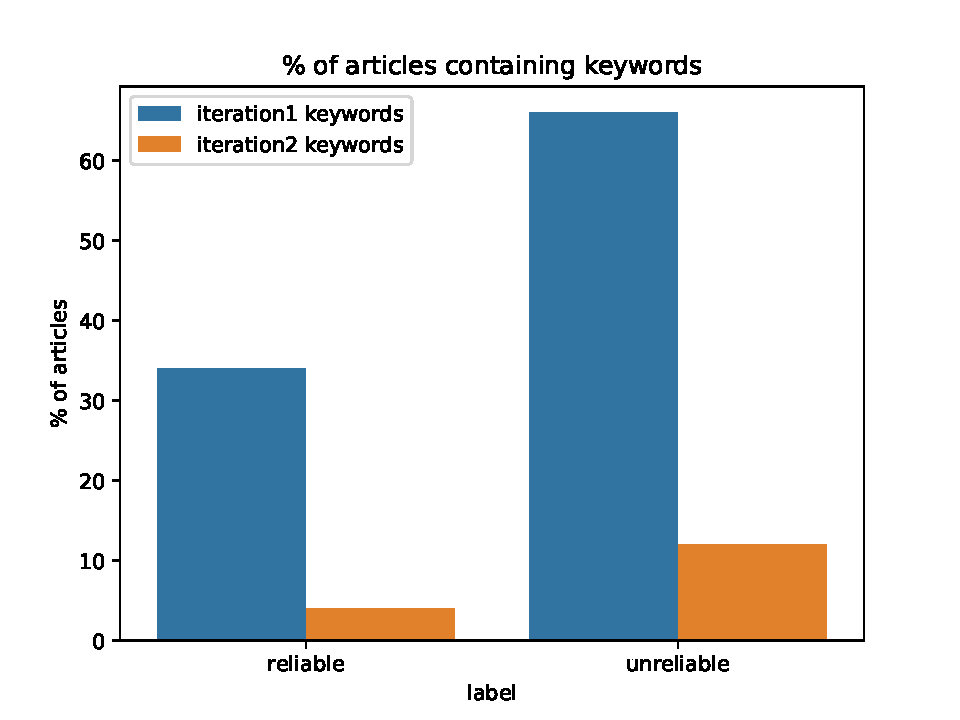
\includegraphics[width=\linewidth]{obrazky-figures/percentage_keywords.pdf}
      \caption{}
      \label{fig:prc_keywords}
    \end{subfigure}%
    \begin{subfigure}{.5\textwidth}
      \centering
      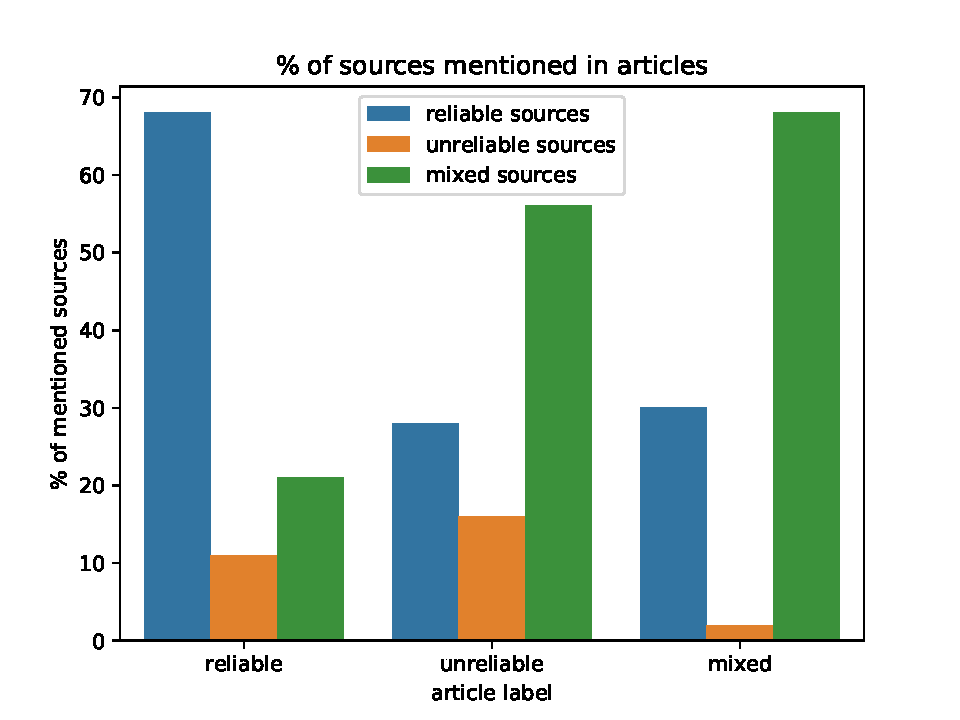
\includegraphics[width=\linewidth]{obrazky-figures/percentage_sources.pdf}
      \caption{}
      \label{fig:prc_sources}
    \end{subfigure}
    \caption{Figure (a) shows the percentage of articles that contained at least one of the filtered keywords. Figure (b) contains the percentage of sources mentioned in reliable unreliable and mixed articles.}
    \label{fig:test3}
\end{figure}

The last step of the preprocessing was creating the train, test and validation splits. The final datasets are presented in table \ref{tab:nela_split}.

\begin{table}[H]
    \centering
\begin{tabular}{|r|r|r|r|}
\hline
\textbf{Dataset} & \textbf{Reliable articles} & \textbf{Unreliable articles} & \textbf{Total} \\ \hline
train & 312,069 & 304,729 & 616,798 \\ \hline
test & 98,337 & 98,103 & 196,440 \\ \hline
validation & 78,851 & 78,346 & 157,197 \\ \hline
\end{tabular}
    \caption{Number of articles in the train, validation and test splits of the NELA dataset.}
    \label{tab:nela_split}
\end{table}


\section{Merged Dataset}
\label{sec:merged}
The NELA dataset, used for training the classifiers, uses source-level labels expanded to all articles. The Merged dataset is used to additionally test the abilities of the classifiers on a dataset whose labels were not extracted from sources. \emph{The Merged dataset was created by merging three fake news datasets with binary labels}: the Fake news dataset described in section \ref{fake_news_dataset}, the Fake or real news dataset described in section \ref{fake_or_real_news} and FakeNewsNet described in section \ref{fake_news_net}. The resulting dataset consists of 27,518 articles (13,769 reliable and 13,749 unreliable). It is intended to be used only for further evaluation of the created classifiers.



\section{Fake News Interpretability Dataset}
\label{test-dataset}
This section introduces the Fake News Interpretability (FNI) dataset created as part of this thesis. It was created for qualitative analysis and evaluation of the implemented classifiers. The FNI dataset consists of 46 manually picked articles (23 reliable, 23 unreliable). For each article, the dataset contains a label, indicating whether it is reliable or unreliable, the URL of the article, the source that published the article, bias and the factuality score of the source (if known) obtained from the MBFC website and the date of publication. The factuality score ranges from 0 (least factual reporting) to 5 (most factual reporting). Table \ref{tab:test_dataset} shows all the fields stored for each article in the dataset.

\begin{table}[H]
    \centering
    \begin{tabular}{c|c|l}
    \textbf{Column} & \cellcolor[HTML]{FFFFFF}\textbf{Type} & \cellcolor[HTML]{FFFFFF}\textbf{Description} \\ \hline
    title      & text & Headline of the article             \\
    text       & text & The text in the body of the article \\
    url        & text & Url of the article                  \\
    label      & text & Binary label (True/Fake)            \\
    source     & text & Source that published the article   \\
    topic      & text & Topic of the article                \\
    mbfc bias  & text & Bias of the source from MBFC        \\
    factuality & text & Factuality of the source from MBFC  \\
    date       & text & Date when the article was published
    \end{tabular}
    \caption{Fields in the FNI dataset.}
    \label{tab:test_dataset}
\end{table}

The fake articles were obtained from three main sources:
\begin{itemize}
    \item The top 50 fake news hits of 2016 published by Buzzfeed News in \cite{buzzfeed:fake}.
    \item The MBFC website --- cherry-picked articles that failed the fact check from several questionable-source, satire and conspiracy-pseudoscience sources.
    \item List of fake news websites at Wikipedia \cite{wiki:fake_list}.
\end{itemize}

Additionally, three fake articles were generated by the ChatGPT\footnote{\url{https://openai.com/blog/chatgpt}} language model. The articles labelled as true were picked from verified factual news published on the following websites:

\begin{itemize}
    \item The MBFC website --- section with verified factual news.\footnote{\url{https://mediabiasfactcheck.com/factual-news/}}
    \item The News Facts Network website --- verified factual news.\footnote{\url{https://newsfactsnetwork.com/}}
\end{itemize}


The MBFC bias and factuality score were explained in section \ref{nela}.
The distribution of biases per label in the FNI dataset is displayed in figure \ref{fig:test_dataset_biases}. The factuality of sources per label in the FNI dataset is shown in figure \ref{fig:test_dataset_fact}.
In cases where the source is not known by the MBFC database, it receives an \texttt{unknown} bias and factuality score. Each article in the dataset also contains a topic. The topic was assigned manually after reviewing each article. It serves mainly informative purposes as the articles were selected with the intention of including various different topics to present enough diversity. The topics were also used to create multiple areas that would test the abilities of the created classifiers. The main areas that were identified are \emph{covid, crime, football, politics, science} and \emph{war}. Each area contains at least two articles for each label (reliable/unreliable). The topics of all articles for each label can be seen in figure \ref{fig:test_dataset_topics}. The analysis of the implemented classifiers on the FNI dataset is described in chapter \ref{chap:inter_anal}. The next chapter discusses the methods proposed to implement the classifiers.

\begin{figure}[H]
    \centering
    \begin{subfigure}{.5\textwidth}
      \centering
      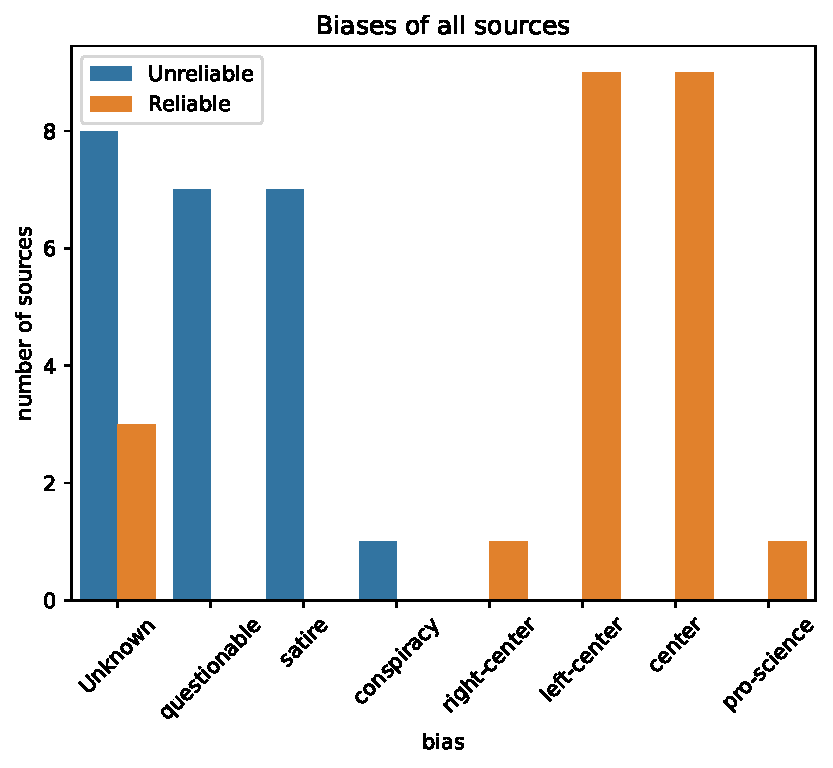
\includegraphics[width=\linewidth]{obrazky-figures/test_dataset_bias_all.pdf}
      \caption{}
      \label{fig:test_dataset_biases}
    \end{subfigure}%
    \begin{subfigure}{.5\textwidth}
      \centering
      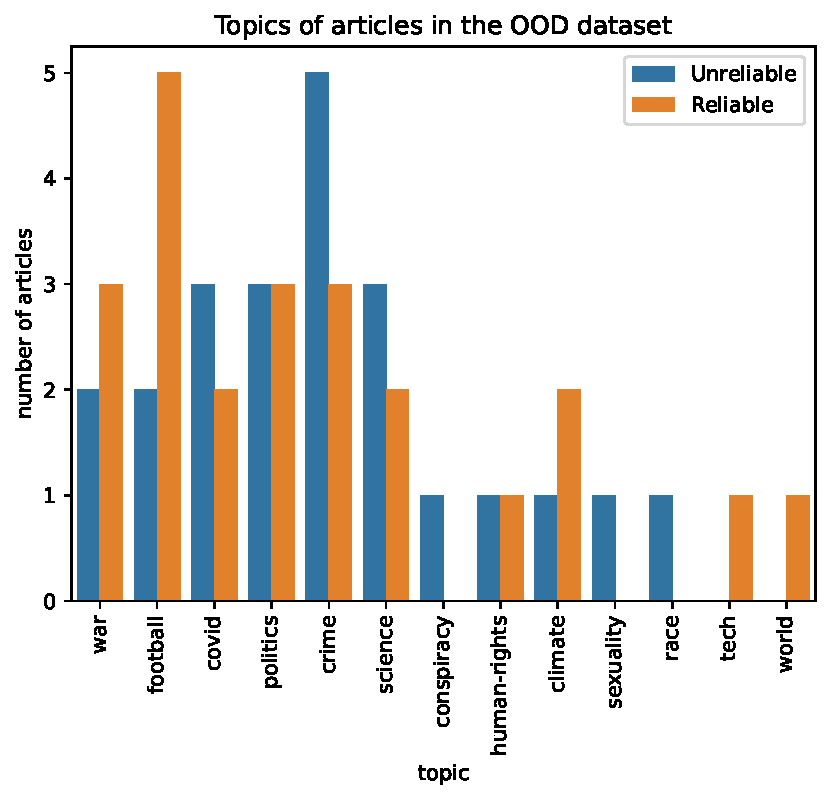
\includegraphics[width=\linewidth]{obrazky-figures/test_dataset_topics.pdf}
      \caption{}
      \label{fig:test_dataset_topics}
    \end{subfigure}
    \caption{Figure (a) shows the number of articles per bias in the FNI dataset. Figure (b) shows the topics of articles in the FNI dataset.}
    \label{fig:test4}
\end{figure}

% The factuality of a source indicates how much are the articles published by this source based on truth. It is a score ranging from 0 (least factual) to 5 (most factual). It is therefore evident, that the articles labelled as fake were published by sources with low factuality and the sources publishing articles labelled as true possess higher factuality scores.

\begin{figure}[]
    \centering
    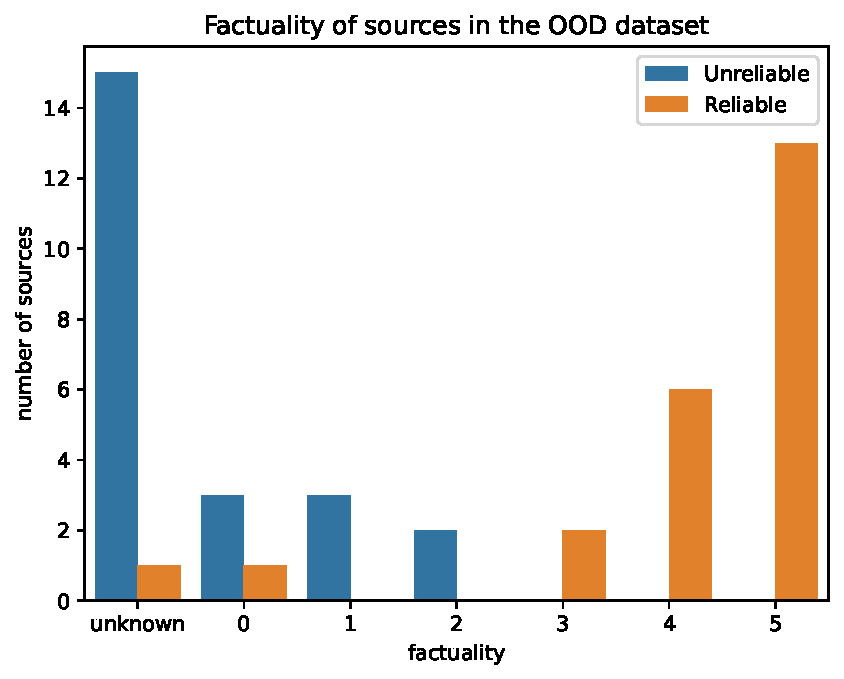
\includegraphics[scale=0.6]{obrazky-figures/test_dataset_factuality.pdf}
    \caption{Number of articles per factuality score in the FNI dataset.}
    \label{fig:test_dataset_fact}
\end{figure}


%%%%%%%%%%%%%%%%%%%%%%%%%%%%%%%%%%
% Proposed Methods
\chapter{Proposed Methods for the Classifiers}
\label{proposed-methods}
This chapter describes the methods used to create the fake news classifiers and obtain predictions in this thesis. In total two different classifiers were created. The first classifier represents the baseline model and is based on a Multinomial Naive Bayes classifier. The second classifier is based on the BERT transformer model and is meant to help better understand the clues exploited in the articles.


\section{Baseline Classifier}
\label{baseline}
The baseline classifier is based on an approach using Term Frequency-Inverse Document Frequency (TF-IDF) and Multinomial Naive Bayes Classifier. This section explains both these methods and describes how they were used in the classifier. Figure \ref{fig:baseline_model} shows the steps in the baseline model. The first step is applying some preprocessing to the input data (news articles). The preprocessing includes removing stop words, URLs and HTML code. Stop words are common words that are considered to be semantically insignificant. Examples of stop words are, e.g., “the”, “a”, “and”, etc. After the preprocessing, TF-IDF is applied to create a feature vector expected as the input for the Multinomial Naive Bayes (MNB) classifier. The MNB classifier then computes the predicted probabilities for each class, i.e., classes reliable and unreliable.

\begin{figure}[H]
    \centering
    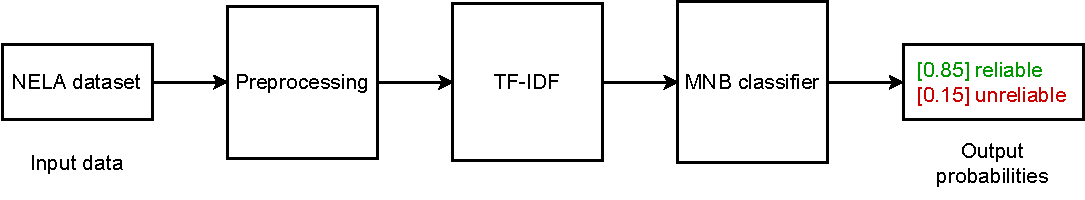
\includegraphics[scale=0.8]{obrazky-figures/baseline_model2.pdf}
    \caption{Steps of the baseline model.}
    \label{fig:baseline_model}
\end{figure}


\subsection*{TF-IDF}
As described in \cite{tf-idf}, TF-IDF is a statistic designed to reflect the importance of a term to a document in a collection of documents (also known as a corpus). It is often used for information retrieval tasks, data mining, recommender systems, as a weighting factor in search engines and other NLP tasks.
The TF-IDF value of a term for a document ranges from 0 to 1. It increases proportionally with the number of times the term appears in the document and decreases with the number of documents in which the term appeared. The computation of TF-IDF is divided into two metrics: Term frequency and Inverse document frequency.

The term frequency of a term represents the significance of the term to a document by the number of its occurrences. The first form of term weighting appeared in \cite{tf}. Term frequency of term $t$ within document $d$ is defined as:

\begin{equation}    
     \operatorname{tf}(t, d) = \displaystyle{\frac{f_{t,d}}{\sum_{t' \in d} f_{t', d}}}
\end{equation}

where $f_{t,d}$ is the number of times term $t$ occurs in document $d$ and the denominator represents the total number of terms in document $d$.

Inverse document frequency, described in \cite{idf}, is a measure of how much information a term provides to a certain document given a corpus of documents. If the term is rare and only appears in one document it is significant for the document. If the term is very common and appears in all documents, its significance and its inverse document frequency are very low. The inverse document frequency of term $t$ to a document $d$ in a corpus of documents $D$ is defined as:

\begin{equation}
     \operatorname{idf}(t, D) =  \operatorname{log} \displaystyle{\frac{N}{|\{d \in D : t \in d\}|}}
\end{equation}

where $N$ is the total number of documents in corpus $D$ meaning $|D| = N$ and the denominator is the number of documents where term $t$ appears. The denominator is often adjusted to $1 + |\{d \in D : t \in d\}|$ to avoid zero division. Finally, the TF-IDF of term $t$ is computed as the product of the two:

\begin{equation}    
     \operatorname{tfidf}(t, d, D) =  \operatorname{tf}(t,d) \cdot  \operatorname{idf}(t, D)
\end{equation}

where $d$ is a document and $D$ is the corpus of documents. The second method used in the baseline system is the Naive Bayes Classifier.

\subsection*{Multinomial Naive Bayes Classifier}
A Naive Bayes Classifier, as described in \cite{bayes} and \cite{bayes-theorem}, is a probabilistic machine learning model for classification tasks. The classifier is based on the Bayes theorem. The Bayes theorem defines the probability of an event based on prior knowledge of conditions that might be related to the event. The theorem is defined by the following equation:

\begin{equation}    
    P(a | b) = \displaystyle{\frac{P(b|a) \cdot P(a)}{P(b)}}
\end{equation}

where $a$, $b$ are realizations of events $A$, $B$ and the probability of $b$ is non-zero: $P(b) \neq 0$. The~following probabilities are used in the theorem:

\begin{itemize}
    \item $P(a | b)$ is the probability of $a$ occurring given that $b$ has occurred (so-called posterior probability in the Bayes formula).
    \item $P(b | a)$ is the conditional probability of $b$ occurring given that $a$ has occurred (so-called likelihood probability in the Bayes formula). 
    \item $P(a)$ is the probability of $a$ occurring (called the prior probability in the Bayes formula).
    \item $P(b)$ is the probability of $b$ occurring (called the evidence or marginal probability in the Bayes formula).
\end{itemize}

Using the explanation given in \cite{colins-mnb} and \cite{naive-bayes-towards}, the Naive Bayes model can be formulated as follows. The classifier uses a labelled training dataset $(\Vec{x}^{(i)}, y^{(i)})$ for $i = 1…n$, where $n$ is the number of samples in the dataset. Each $\Vec{x}^{(i)}$ is a $d$-dimensional vector, where $d$ specifies the number of features in the~model and each $y^{(i)}$ is in $\{1,2,...,k\}$, where $k$ is the number of classes in the problem. In the case of a binary classifier $k = 2$. 
Considering the problem of classifying fake news articles into two different classes (reliable, unreliable) the Multinomial Naive Bayes classifier is used. The label $y^{(i)}$ represents the class of the $i$-th article in the training set. With the approach of using word counts (or TF-IDF), $d$ corresponds to the vocabulary size in the corpus --- the total number of unique words in the dataset. Each component of the vector of features $\Vec{x}^{(i)}_j$ for $j = 1…d$, contains a number that represents the number of occurrences (or the TF-IDF value) of the $j$-th word in the $i$-th article. 

The Naive Bayes classifier assumes the features in the model are independent. That means the presence of one particular feature does not affect the other features. Hence it is called naive. Another assumption made by the model is that all the features have an equal effect on the outcome. This means they all affect the result equally. The Naive Bayes model is then derived as follows. 

\begin{equation}
    P(y | \Vec{x}) = \displaystyle{\frac{P(\Vec{x}|y) \cdot P(y)}{P(\Vec{x})}}
\end{equation}

where $y$ corresponds to the label $y^{(i)}$ and $\Vec{x}$ corresponds to the feature vector $\Vec{x}^{(i)}$. As the model assumes that all features are independent, the probability $P(\Vec{x}|y)$ can be computed as the product of the separate probabilities for each feature.

\begin{equation}    
    P(y | x_1, ..., x_d) = \displaystyle{\frac{P(x_1|y) P(x_2|y) ... P(x_d|y) P(y)}{P(x_1) P(x_2)...P(x_d)}}
    \label{eq:mnb1}
\end{equation}

where $d$ is the number of features in the model. For all entries in the dataset, the denominator does not change, it remains static. Therefore, the equation \ref{eq:mnb1} can be reformulated using proportionality.

\begin{equation}
    P(y|x_1, ..., x_d) \propto P(y) \prod_{j=1}^d P(x_j|y)
\end{equation}

In the case of a binary fake news classifier, the class variable $y$ has only two outcomes. The classification is then performed by finding the class with the maximum probability.

\begin{equation}    
    y = \underset{y\in\{1,..,k\}}{\arg\max} \; P(y) \prod_{j=1}^d P(x_j|y)
\end{equation}

where $k=2$ for a binary classifier. The probabilities in the equation are estimated from the data using the maximum-likelihood estimates for the Naive Bayes model. The probability $P(y)$ can be interpreted as the probability of seeing the label y in the data. The maximum-likelihood estimates for $P(y)$, where $y \in {1…k}$ take the following form.

\begin{equation}
    P(y) = \displaystyle{\frac{\sum_{i=1}^n \mathbb{I}[y^{(i)} = y]}{n} = \frac{\operatorname{count}(y)}{n}}
    \label{eq:ml1}
\end{equation}

where $n$ is the number of samples (articles) in the dataset and $\mathbb{I}[y^{(i)} = y]$ is defined as $1$ if $y^{(i)} = y$, $0$ otherwise. Therefore, $\sum_{i=1}^n \mathbb{I}[y^{(i)} = y]$ corresponds to the number of times label $y$ appears in the dataset. As the equation \ref{eq:ml1} shows, the probability of $P(y)$ is simply the number of times the label $y$ appears in the dataset divided by the number of samples in the dataset. 

The other probability that needs to be estimated is the $P(x_j|y)$ for each feature $j \in d$ in vector $\Vec{x}$. This probability can be understood as the probability of feature $x_j$ appearing in a sample belonging to class $y$. The ML estimates for $P(x_j|y)$ depend on the distribution of the training data. In the case of a Multinomial Naive Bayes classifier, the ML estimates take the following form.

\begin{equation}
    P(x_j|y) = \displaystyle{\frac{\sum_{i=1}^n \mathbb{I}[y^{(i)} = y] \; x_j^{(i)}}{\sum_{i=1}^n \sum_{t=1}^d \mathbb{I}[y^{(i)} = y] \; x_t^{(i)}} = \frac{\operatorname{N}_{yj}}{\operatorname{N}_y}}
    \label{eq:ml2}
\end{equation}

where $n$ is the number of samples in the dataset, $\operatorname{N}_{yj}$ is the is the number of times feature $j$ appears in a sample of class $y$ in the training dataset and $\operatorname{N}_y$ is the total count of all features for class $y$. In the case of using TF-IDF values the equation just sums the TF-IDF values of features instead of the discrete counts of their occurrence. The equation \ref{eq:ml2} is often adjusted by adding a smoothing prior $\alpha \geq 0$. The smoothing accounts for features not present in the training samples and prevents zero probabilities in the computation. Setting $\alpha = 1$ is called Laplace smoothing and when $\alpha < 1$ it is called the Lidstone smoothing. 

\begin{equation}
    P(x_j|y) = \displaystyle{\frac{N_{yj} + \alpha}{N_y + \alpha d}}
    \label{eq:ml_estimates}
\end{equation}

where $d$ is the number of features in the model. During the inference of new articles, the new TF-IDF values of these articles are used as an exponent of the trained probabilities as described in equation \ref{eq:infer-prob}.

\begin{equation}
    P(y|\Vec{x}) = \displaystyle{\frac{P^{'}(\Vec{x}|y) \cdot P(y)}{\sum_y{P^{'}(\Vec{x}|y) \cdot P(y)}}}
    \label{eq:infer-prob}
\end{equation}

where $P^{'}$ is the distribution exponentiated by the new TF-IDF values. The Multinomial Naive Bayes classifier is intended to be used with integer feature (word) counts. However, TF-IDF vectors are also known to work well in practice. Both approaches --- the word counts and TF-IDF vectors --- were tried and compared in this thesis and the approach of using TF-IDF was found to perform slightly better. This comparison is further described in chapter \ref{experiments}. 

In this thesis, the scikit-learn\footnote{\url{https://scikit-learn.org/stable/modules/naive_bayes.html\#multinomial-naive-bayes}} implementation of the MNB classifier is used. This implementation uses the formula described in equation \ref{eq:ml_estimates} to compute the ML estimates.
Among the advantages of a Naive Bayes Classifier is the speed of computation and ease of implementation. The disadvantage of this model is the fact that all features are considered independent. In reality, words have relations with each other and are often part of a broader context. To solve these problems the BERT transformer model is proposed in the next section. 


%on the other hand, include the equality of features (meaning all features influence the outcome of the classifier equally)




\section{BERT Classifier}
\label{sec:bert}
This section describes the second classifier implemented in this thesis. The architecture chosen for the second classifier is the BERT model. The baseline classifier models the documents based only on the occurrence of words without any deeper understanding of the text. A~better approach is using word embeddings that are trained to capture the relationships between words based on their co-occurrence in a document and convey the meaning of words to allow for deeper understanding. The BERT model uses contextualized embeddings where the embedding of a word depends on the context of the sentence in which it occurs.
The BERT (Bidirectional Encoder Representations from Transformers) model, introduced in \cite{bert}, is a language representation model that produces state-of-the-art results in a wide variety of NLP tasks. The model utilizes the approach of transfer learning --- pre-training a neural network model and fine-tuning it for specific tasks. This means BERT was designed to pre-train deep bidirectional representations from unlabeled text and then fine-tune the pre-trained model on a downstream task. During the fine-tuning, the model is first initialized with the pre-trained parameters. All parameters are then fine-tuned using labelled data, e.g., by adding one additional output layer to the model.
The architecture of BERT is based on the Transformer architecture described in \cite{transformer}. The Transformer architecture uses the encoder-decored structure displayed in figure \ref{fig:transformer}.

\begin{figure}[H]
    \centering
    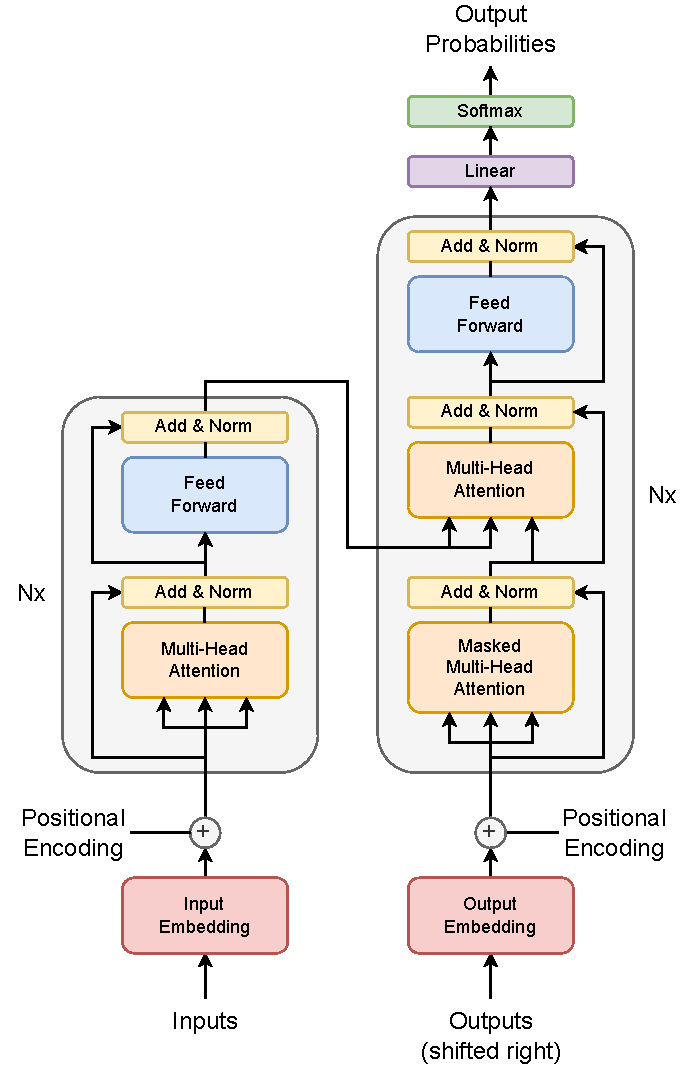
\includegraphics[scale=0.7]{obrazky-figures/transformer.pdf}
    \caption{Architecture of the Transformer model, as described in \cite{transformer}.}
    \label{fig:transformer}
\end{figure}

The encoder takes an input sequence (e.g., a sentence in English) and computes its hidden representation. This hidden representation is then used by the decoder to generate the desired output sequence of symbols one element at a time (e.g., the input sentence translated to French). As the decoder generates the output it uses the previously generated symbols as additional input when generating the next symbol. This transformation of an input sequence to an output sequence makes the model suitable for applications like translation, question answering, text summarization, etc.

Each word in the input sentence is first transformed into the input embedding 512-dimensional vector, to which positional encoding is added. The positional encoding is a vector that helps to determine the position of words in the sentence. After that the vectors are passed into the first layer of the encoder. The original paper uses a stack of $N=6$ layers in the encoder connected in a sequence. Each layer contains two components: a multi-head self-attention mechanism and a feed-forward neural network.

\subsection*{Multi-head Attention}
The self-attention mechanism helps the model determine the relevance between words in the input sentence. As the model processes each word, the self-attention allows it to look at the other words and based on their relevance to the processed word contribute to a better encoding for this word. For example, when the model processes this sentence: “The animal didn't cross the street because it was too tired”, self-attention allows the model to associate the word “it” with the word “animal”.

The self-attention mechanism works as follows. First, each input vector of the encoder (the word embeddings in the first layer) is transformed into three vectors: Query vector $q$ and Key vector $k$ of dimensions $d_k$, and Value vector $v$ of dimension $d_v$. These vectors are created by multiplying the input embedding with three weight matrices $W_Q$, $W_K$, and $W_V$ that are trained during the training process, as displayed in figure \ref{fig:attention1}.

\begin{figure}[H]
    \centering
    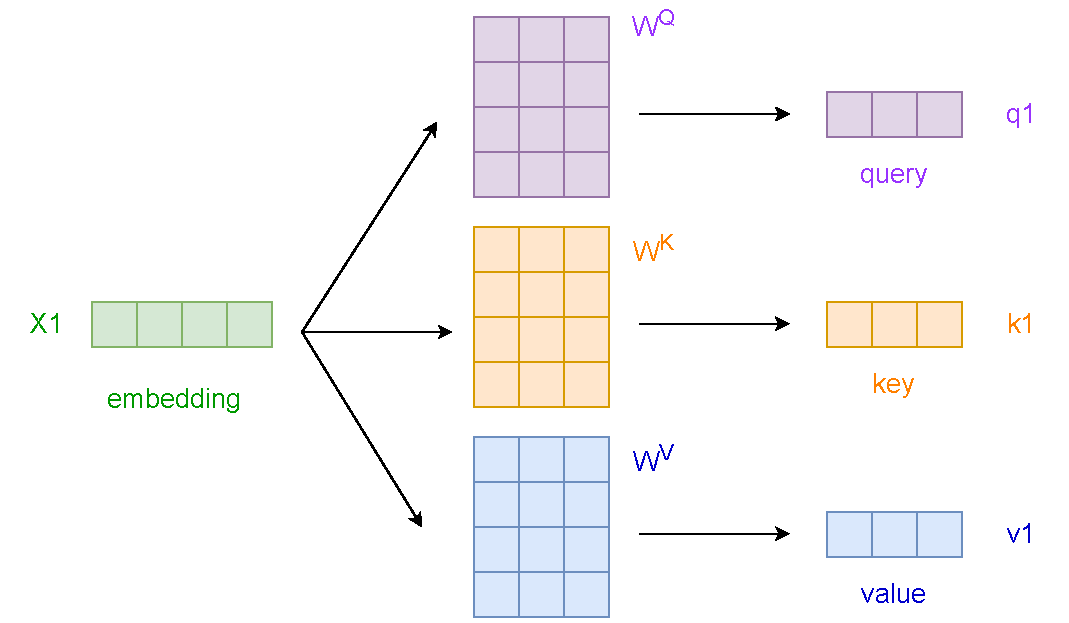
\includegraphics[scale=0.6]{obrazky-figures/attention1.pdf}
    \caption{Creation of the query, key and value vectors from the input embedding by multiplying the embedding with weight matrices trained during the training process (biases omitted for simplicity).}
    \label{fig:attention1}
\end{figure}


To compute the attention vector for a word at position $i=1$ with all the other words $j\in1...t$ where $t$ is the number of words in the sentence, the model computes the dot product of query $q_i$ with each key $k_j$, divides the result by $\sqrt{d_k}$ and applies the $\operatorname{softmax}$ function to obtain the weights of the values. After that, each value vector $v_j$ is multiplied by the corresponding $\operatorname{softmax}$ value to obtain a weighted value vector. In the last step, all the weighted value vectors are summed to create one attention vector $z_i$ for word $i$. This process is shown in figure \ref{fig:attention2}.

\begin{figure}[H]
    \centering
    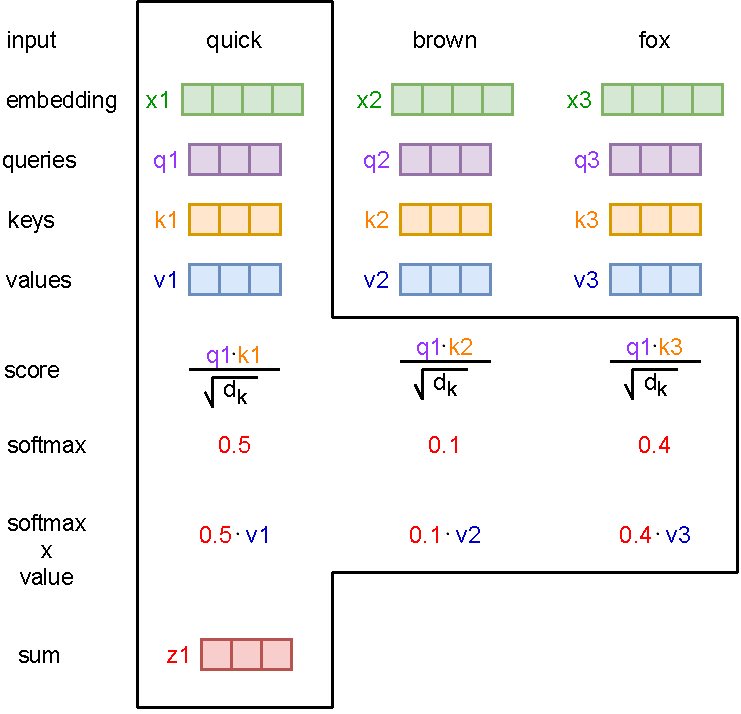
\includegraphics[scale=0.8]{obrazky-figures/attention2.pdf}
    \caption{Computation of the attention vector $z$ for a word in a sequence, as described in The Illustrated Transformer \cite{illustrated-transformer}.}
    \label{fig:attention2}
\end{figure}


In practice, the input vectors, their queries, keys and values are all packed together into matrices and the attention function is computed for a set of queries simultaneously. The attention of a query matrix $Q \in \mathbb{R}^{L \times d_k}$, a key matrix $K \in \mathbb{R}^{L \times d_k}$ and a value matrix $V \in \mathbb{R}^{L \times d_v}$ --- where $d_k$ is the dimension of the query and key vectors and $d_v$ is the dimension of the value vector --- can be represented by equation \ref{eq:attention}.

\begin{equation}
    \operatorname{Attention}(Q, K, V) = \operatorname{softmax} \displaystyle{(\frac{QK^T}{\sqrt{d_k}})V}
    \label{eq:attention}
\end{equation}

where $d_k$ is the dimension of the query and key vectors (64 in the original paper). The process described above is the computation of a single attention function. The Transformer model uses Multiple-head attention. Each attention head contains its own weight matrices $W_Q$, $W_K$, $W_V$ and computes the attention matrix $Z_i$. The matrices from all heads are then concatenated together and multiplied by another weight matrix $W^0$ trained jointly with the model. After that, the flow continues to the second component of the transformer --- a feed-forward neural network --- which is applied to every one of the attention vectors. Around each of the components, there is a residual connection followed by layer normalization. 

The decoder is also composed of $N=6$ identical layers. The input for the decoder is actually the desired output of the transformer (e.g., a sentence translated into another language). The BERT model uses only the encoder, therefore, the decoder is not further described in this section.
% The output is first transformed into embeddings and positional encoding is added. After that masked multi-head self-attention is applied. In this case, the self-attention just masks the words that follow later in the sequence which ensures that the prediction for position $i$ depends only on the known words that came before $i$. After that another multi-head self-attention is applied, this time combining the outputs of the encoder with the decoder. This is where the mapping between English and French words (in the example of language translation) takes place. The last component of the decoder is once again a feed-forward neural network. The decoder employs residual connections and normalization just like the encoder. Finally, after a linear layer followed by softmax, the transformer generates the output probabilities.

\subsection*{BERT model}
The BERT model used in this thesis is based on the Transformer described above. The architecture of BERT is a multi-layer bidirectional Transformer encoder as it uses only the encoder part of the transformer. Authors of the BERT model created two pre-trained versions: $\operatorname{BERT_{BASE}}$ and $\operatorname{BERT_{LARGE}}$. The $\operatorname{{BERT_{BASE}}}$ model used in this thesis contains 12 encoder blocks and 110 million parameters.
The BERT model is pre-trained on two unsupervised tasks: Masked Language Model (MLM) and Next Sentence Prediction (NSP).

MLM is used to train bidirectional representations. A percentage of the input tokes is masked at random --- they are replaced by the [MASK] token. The model then learns to predict the masked words from the context words on either side of the sequence. This is achieved by adding a classification layer at the end of the encoder and performing a softmax over the vocabulary. A downside to this approach is that the [MASK] token is not used during fine-tuning. Therefore the [MASK] token is only used in 80\% of the randomly selected tokens, 10\% is replaced by a random token and the remaining 10\% stays unchanged. During the training, a cross-entropy loss is used.

In NSP the model is fed pairs of sentences $A$, $B$ and learns to predict whether sentence $B$ is subsequent to sentence $A$ in the original document. In 50\% of the pairs used for training, $B$ is subsequent to $A$ and in the other 50\%, $B$ is a random sentence not subsequent to sentence $A$. Both sentences are fed into the model as one input sequence. Each sequence starts with the [CLS] token, followed by tokens of sentences $A$ and $B$ separated by the [SEP] token. The model then takes the token embeddings of each word and adds a segment embedding, indicating to which sentence the given word corresponds, and a position embedding, that indicates the position of each word in the sequence. Figure \ref{fig:bert1} provides a visual illustration of the BERT input representation.

\begin{figure}[H]
    \centering
    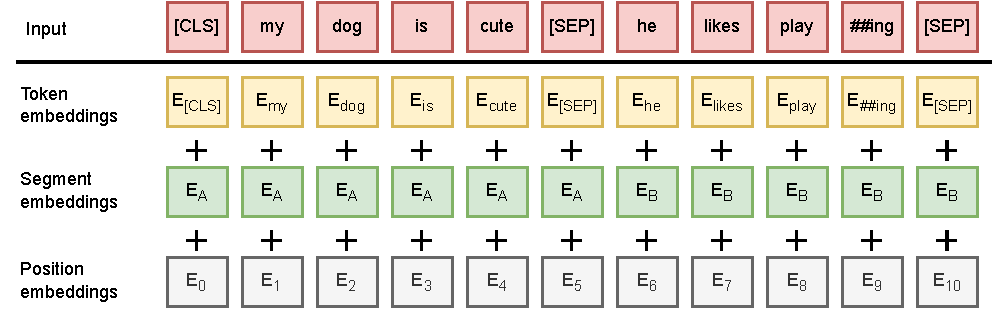
\includegraphics[scale=0.8]{obrazky-figures/bert1.pdf}
    \caption{Representation of BERT input is the sum of token embeddings, segmentation embeddings and position embeddings, as described in \cite{bert}.}
    \label{fig:bert1}
\end{figure}

When training the model the MLM and NSP are trained together. To predict whether the sentence $B$ is subsequent to $A$ the model adds a classification layer on top of the encoder output for the [CLS] token and computes the probability with softmax.

This thesis uses the $\operatorname{{BERT_{BASE}}}$ uncased model that was pre-trained on the BooksCorpus (800M words) \cite{book_corpus} and English Wikipedia (2,500M words). The model is then fine-tuned on the NELA dataset described in section \ref{nela-my}, which contains binary labels representing whether the given article is reliable or unreliable. For fine-tuning, a classification layer is added on top of the encoder output for the [CLS] token. The classification layer is simply a linear layer with dropout and optionally some activation function, e.g., ReLU. The linear layer has 768 input features (hidden size of $\operatorname{{BERT_{BASE}}}$) and 2 output features (number of labels in the dataset). The fine-tuning process is displayed in figure \ref{fig:bert2}.

\begin{figure}[H]
    \centering
    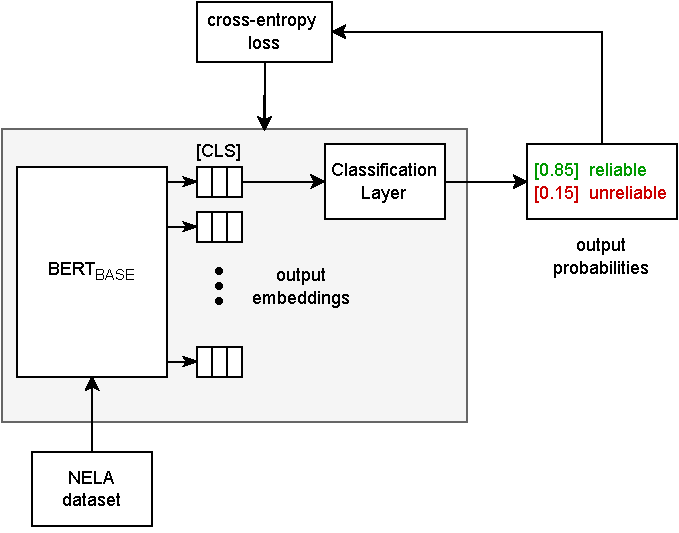
\includegraphics[scale=0.9]{obrazky-figures/bert2.pdf}
    \caption{Fine-tuning the $\operatorname{BERT_{BASE}}$ model on the NELA dataset.}
    \label{fig:bert2}
\end{figure}



\section{Interpretability with Integrated Gradients}
\label{sec:integ_grads}
This section describes the method used for gaining interpretable cues from the BERT classifier. Due to the deep stack of layers used in models like BERT, deep neural networks are often viewed as black boxes in the sense that it is not simple to interpret the predictions they generate. However, it is possible to implement a method able to interpret the predictions of neural networks. An interpretation method like this seeks to answer the following questions: (i) Why does the model predict the given class? (ii) What are the features exploited by the model during the prediction (i.e., what are the most important words that influence the prediction)?

To gain interpretable cues from the BERT classifier the Integrated gradients (IG) method is used in this thesis. Integrated gradients, presented in \cite{integ_grads}, is a method that requires no modification to the original network. It is simple to implement and can be applied to any deep-learning model for classification and regression tasks. The method computes an attribution score for each input feature of the deep learning model based on the gradients of the output prediction. Following is the formal definition of the method, as defined in \cite{integ_grads}.

\vspace{2mm}

\textbf{Definition:} Suppose a function $F: \mathbb{R}^n \rightarrow [0, 1]$ that represents a deep network and a~vector $\Vec{x} = (x_1, …, x_n)$ representing an input. An attribution of the prediction at input $\Vec{x} \in \mathbb{R}^n$ relative to a baseline input $\Vec{x}^{'} \in \mathbb{R}^n$ is a vector $\Vec{a}_F(\Vec{x}, \Vec{x}^{'}) = (a_1, …, a_n) \in \mathbb{R}^n$ where each $a_i$ is the contribution of $x_i$ to the prediction for $F(\Vec{x})$.

\vspace{2mm}

The vector $\Vec{x}$ is used as the input of the neural network for simplicity as usually the input of a neural network is a matrix. The Integrated gradients method requires two sets of input: the original input and a baseline input. The original input corresponds to the unchanged input $\Vec{x}$ of the network. The baseline input is constructed from the original input and should contain neutral values. As suggested by the authors of the original paper, for image processing, the baseline could be a black image, whereas for text models it could be a zero embedding vector. In practice, the [PAD] token is often used in the baseline input, as it is interpreted by the network as empty space (even though it does not have zero embeddings). The difference between the original and baseline input is also described in figure \ref{fig:integ_grads1}.

\begin{figure}[H]
    \centering
    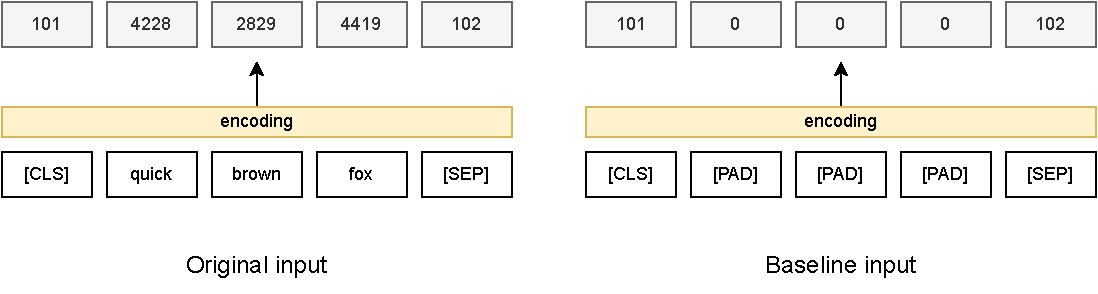
\includegraphics[scale=0.8]{obrazky-figures/integ_grads1.pdf}
    \caption{Example of the input and baseline text used in the Integrated gradients method as described in \cite{integ_grads_towards}.}
    \label{fig:integ_grads1}
\end{figure}

The Integrated gradients are defined as the integral of the gradients along a straight line path (in $\mathbb{R}^n$) from the baseline $\Vec{x}^{'}$ to the original input $\Vec{x}$. The Integrated gradient of the $i^{th}$ dimension for an input $\Vec{x}$ and a baseline input $\Vec{x}^{'}$ is defined in equation \ref{eq:integ_grads1}.

\begin{equation}
    \operatorname{IntegratedGrads}_i(\Vec{x}) = (x_i - x^{'}_i) \cdot \int_{\alpha = 0}^{1} \displaystyle{\frac{\partial F(\Vec{x}^{'} + \alpha \cdot (\Vec{x}-\Vec{x}^{'}))}{\partial x_i}} d\alpha
    \label{eq:integ_grads1}
\end{equation}

where $\frac{\partial F(\Vec{x})}{\partial x_i}$ is the gradient of $F(\Vec{x})$ along the $i^{th}$ dimension. In practice, the integral of Integrated gradients can be approximated as the sum of the gradients at multiple points occurring at sufficiently small intervals on the straight line between $\Vec{x}^{'}$ and $\Vec{x}$. This technique is also known as the Riemann sum. It is the sum of the gradients divided by the number of approximation steps. Equation \ref{eq:integ_grads1} can be therefore approximated as:

\begin{equation}
    \operatorname{IntegratedGrads}^{approx}_i(\Vec{x}) = (x_i - x^{'}_i) \cdot \sum_{k=1}^{m} \displaystyle{\frac{\partial F(\Vec{x}^{'} + \frac{k}{m} \cdot (\Vec{x} - \Vec{x}^{'}))}{\partial x_i}} \cdot \frac{1}{m}
    \label{eq:integ_grads2}
\end{equation}

where $m$ is the number of approximation steps. In the case of the BERT classifier used in this thesis, function $F$ represents the classifier model. The model predicts the probabilities of two classes, therefore one target probability, e.g., probability of class \texttt{reliable}, is selected to be the output of $F$. The input $\Vec{x}$ represents the text of an article and $x_i$ represents each word. The IG method gradually interpolates the baseline input $\Vec{x}^{'}$ to move closer to the original input --- by increasing the $k$ value in each approximation step --- and feeds it into the network. This is achieved by the following part of the equation: $(\Vec{x}^{'} + \frac{k}{m} \cdot (\Vec{x} - \Vec{x}^{'}))$.
In the last step when $k=m$ the interpolated input is identical to the original input. The interpolated inputs are gradually fed into the network and in each step, the gradient of $F$ along the $i^{th}$ dimension is computed. 
The formula computes the attribution score for each embedding element. The BERT classifier used in this thesis uses 768-dimensional embeddings. Therefore the final attribution score of the $i^{th}$ word is computed as the attribution average of all of the embedding elements. The attribution score is computed for all words in the text as displayed in figure \ref{fig:integ_grads2}.

\begin{figure}[H]
    \centering
    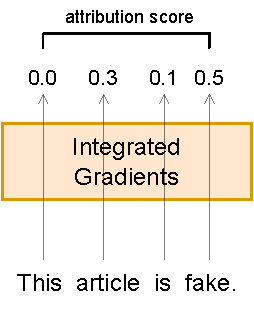
\includegraphics[scale=1]{obrazky-figures/ig.pdf}
    \caption{Application of Integrated gradients as described in \cite{integ_grads_towards}.}
    \label{fig:integ_grads2}
\end{figure}

The method of Integrated gradients is used to get an insight into the predictions of the BERT classifier and explore which features of the text are exploited by the model when making predictions. Chapter \ref{chap:inter_anal} describes the qualitative analysis of the created classifiers using the IG method.


%%%%%%%%%%%%%%%%%%%%%%%%%%%%%%%%%%
% Technical Details
\section{Technical Details}
\label{implementation}
This section provides a brief discussion of the tools and libraries used to implement the models in this thesis. All models are implemented in Python 3.9.7. The implementation of the baseline model uses the Python scikit-learn\footnote{\url{https://scikit-learn.org/stable/}} library. Two main classes are used by the baseline. The TfidfVectorizer is used to convert a collection of input articles to a matrix of TF-IDF features. The MultinomialNB class is an implementation of the Naive Bayes classifier for multinomial models and is used as the classifier in the baseline. Both classes can be found on the scikit-learn website. 

The BERT classifier uses the Hugging Face framework. In particular the pre-trained BERT base uncased model\footnote{\url{https://huggingface.co/bert-base-uncased}}. For the implementation of Integrated gradients, the Layer Integrated Gradients\footnote{\url{https://captum.ai/api/layer.html\#layer-integrated-gradients}} class from the Captum library is used. The usage of this class is based on an explanation in \cite{integ_grads_towards}.





%%%%%%%%%%%%%%%%%%%%%%%%%%%%%%%%%%
% Experiments
\chapter{Quantitative Analysis of the Classifiers}
\label{experiments}
This chapter summarizes the quantitative evaluation of the classifiers implemented in this thesis. The intention is to evaluate the performance of the Baseline classifier and the BERT classifier by applying various evaluation metrics and to analyse their biases in certain areas. To test the implemented classifiers, the following evaluation process was used:

\begin{enumerate}
    \item Train the classifier on a split of the NELA dataset (train set).
    \item Tune the hyper-parameters of the model using the validation split of the NELA dataset (validation set).
    \item Evaluate the classifier on the test split of the NELA dataset (test set).
    \item Perform cross-evaluation of the classifier on the Merged dataset.
    \item Perform cross-evaluation of the classifier on the FNI dataset.
\end{enumerate}

The evaluation of the classifiers is performed using four evaluation metrics: accuracy, precision, recall and F1-score. Following is a brief explanation of these methods.

\subsection*{Confusion Matrix}
To understand the evaluation metrics it is first important to introduce the confusion matrix. A confusion matrix as described in \cite{confusion_matrix}, is a square matrix that is used to evaluate the performance of machine learning algorithms in classification tasks. Each row of the matrix represents the instances in the actual class while each column represents the instances predicted by the model.

\begin{figure}[H]
    \centering
    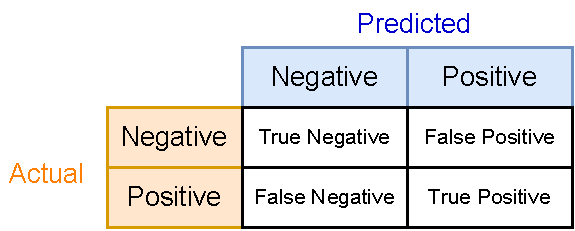
\includegraphics[scale=0.9]{obrazky-figures/conf_mat2.pdf}
    \caption{Example of a confusion matrix for a binary classifier.}
    \label{fig:conf_mat}
\end{figure}

In the case of a binary classifier with only two classes (negative and positive), the confusion matrix would look as displayed in figure \ref{fig:conf_mat}.
The numbers in the cells have specific names. True negative (TN) is the number of instances of class negative that were correctly predicted as negative. False negative (FN) is the number of instances of class positive that were mistakenly classified as negative. False positive (FP) is the number of negative instances falsely predicted to be positive. True positive (TP) is the number of instances correctly classified as positive.


\subsection*{Accuracy}
Accuracy is defined as the number of correctly predicted instances divided by the total number of instances in the dataset (confusion matrix). Using the terms of the confusion matrix it could be also defined as:

\begin{equation}
    Accuracy = \displaystyle{\frac{TN + TP}{TN + FP + TP + FN}}
\end{equation}

Accuracy is often used together with other metrics --- precision and recall --- to better reflect the capabilities of the classifier.

\subsection*{Precision}
Precision is defined as the number of correctly predicted instances of one class divided by the total number of predictions of that class. Equation \ref{eq:precision} shows the definition in terms of the confusion matrix for class positive.

\begin{equation}
    \label{eq:precision}
    Precision = \displaystyle{\frac{TP}{TP + FP}}
\end{equation}

Precision is a good measure to determine the performance of a model where the cost of a false positive (FP) is high. For example, in a fake news classifier, the positive class could be interpreted as fake news and the negative as true (not fake news). In that case, a false positive would be a non-fake news article falsely classified as fake news. A model with too many false positives would receive a low precision.


\subsection*{Recall}
Recall is defined as the number of correctly predicted instances of one class divided by the total number of actual instances of that class, as displayed in equation \ref{eq:recall}.

\begin{equation}
    \label{eq:recall}
    Recall = \displaystyle{\frac{TP}{TP + FN}}
\end{equation}

Recall is crucial for models with a big risk associated with false negatives (FN). In the case of a fake news classifier, false negatives would be fake news articles that are falsely classified as true. In this case, the cost of such a prediction may be harmful but not catastrophic. But for a classifier predicting whether a bank transaction is fraudulent, the consequence of false negative cases could be very bad for the bank.

\subsection*{F1-score}
F1-score is a function of precision and recall. It is defined using the following formula.

\begin{equation}
    F1 = 2 \cdot \displaystyle{\frac{Precision \cdot Recall}{Precision + Recall}}
\end{equation}

The F1 score is beneficial for finding a balance between precision and recall and for datasets with an uneven class distribution.



\section{Evaluation on the NELA Test Set}
\label{sec:eval_nela}
This section describes the evaluation of the baseline and BERT classifiers on the test split of the NELA  dataset. A detailed description of the NELA dataset and its preprocessing can be found in sections \ref{nela} and \ref{nela-my}. Table \ref{tab:nela_val_test} shows the number of articles in the train, test and validation splits. The distribution of labels is well-balanced with all splits having an accuracy around 50\% for majority and random classifiers.

\begin{table}[H]
    \centering
\begin{tabular}{r|r|r|r|}
\cline{2-4}
\multicolumn{1}{c|}{} & \multicolumn{1}{c|}{\textbf{Reliable}} & \multicolumn{1}{c|}{\textbf{Unreliable}} & \multicolumn{1}{c|}{\textbf{Total}} \\ \hline
\multicolumn{1}{|r|}{\textbf{Train}}      & 312,069 & 304,729 & 616,798 \\ \hline
\multicolumn{1}{|r|}{\textbf{Test}}       & 98,337  & 98,103  & 196,440 \\ \hline
\multicolumn{1}{|r|}{\textbf{Validation}} & 78,851  & 78,346  & 157,197 \\ \hline
\end{tabular}
    \caption{Number of reliable and unreliable articles in the train, test and validation splits of the NELA dataset.}
    \label{tab:nela_val_test}
\end{table}

The architecture of the baseline classifier combines the TF-IDF method with a Multinomial Naive Bayes (MNB) classifier and was described in section \ref{baseline}.
Different configurations of the baseline model were examined in order to leverage its capabilities. Multinomial Naive Bayes (MNB) is often used with just word counts instead of TF-IDF. Table \ref{tab:baseline_tf-idf} shows the comparison of using word counts and TF-IDF in the baseline classifier.
The table shows the precision, recall and F1-score for each label and the overall accuracy. As the results show, the usage of TF-IDF slightly improved the classifier. 

\begin{table}[H]
    \centering
\begin{tabular}{cc|c|c|c|}
\cline{3-5}
                                        &                     & \textbf{Precision} & \textbf{Recall} & \textbf{F1-score} \\ \hline
\multicolumn{1}{|c|}{\multirow{3}{*}{Word counts}} & \textbf{Reliable}   & 0.77               & 0.80            & 0.78              \\ \cline{2-5} 
\multicolumn{1}{|c|}{}                  & \textbf{Unreliable} & 0.80               & 0.76            & 0.78              \\ \cline{2-5} 
\multicolumn{1}{|c|}{}                  & \textbf{Accuracy}   & \multicolumn{3}{c|}{0.78}                                \\ \hline \hline
\multicolumn{1}{|c|}{\multirow{3}{*}{TF-IDF}} & \textbf{Reliable}   & 0.79               & 0.80            & 0.80              \\ \cline{2-5} 
\multicolumn{1}{|c|}{}                  & \textbf{Unreliable} & 0.80               & 0.78            & 0.79              \\ \cline{2-5} 
\multicolumn{1}{|c|}{}                  & \textbf{Accuracy}   & \multicolumn{3}{c|}{0.79}                                \\ \hline
\end{tabular}
    \caption{Comparison of using word counts and TF-IDF in the baseline classifier.}
    \label{tab:baseline_tf-idf}
\end{table}

The TF-IDF classifier achieved an accuracy of 79\%. When using the word counts, the accuracy dropped to 78\%. An improvement in the performance of the baseline was achieved when the TF-IDF values were computed using not only words (unigrams) but also bigrams and trigrams. A bigram is a sequence of two adjacent words in a sentence and a trigram is a sequence of three adjacent words. This approach improved the accuracy of the model to 86\%. Table \ref{tab:baseline_trigrams} shows the evaluation results of this approach.


\begin{table}[H]
    \centering
\begin{tabular}{c|ccc|}
\cline{2-4}
 & \multicolumn{1}{c|}{\textbf{Precision}} & \multicolumn{1}{c|}{\textbf{Recall}} & \textbf{F1-score} \\ \hline
\multicolumn{1}{|c|}{\textbf{Reliable}} & \multicolumn{1}{c|}{0.84} & \multicolumn{1}{c|}{0.89} & 0.86 \\ \hline
\multicolumn{1}{|c|}{\textbf{Unreliable}} & \multicolumn{1}{c|}{0.88} & \multicolumn{1}{c|}{0.82} & 0.85 \\ \hline
\multicolumn{1}{|c|}{\textbf{Accuracy}} & \multicolumn{3}{c|}{0.86} \\ \hline
\end{tabular}
    \caption{Baseline with TF-IDF, unigrams, bigrams and trigrams evaluated on the NELA test set.}
    \label{tab:baseline_trigrams}
\end{table}


Adding bigrams and trigrams, however, dramatically increased the memory usage of the model making it much slower. Table \ref{tab:mem_comp} compares the corpus size of the two approaches. The corpus size represents the number of features of the model. For the baseline model using only words (unigrams), the corpus size is equal to the number of all unique words in the dataset. For the model with words, bigrams and trigrams the corpus size is enlarged by the number of unique bigrams and trigrams.

\begin{table}[H]
    \centering
\begin{tabular}{|c|r|}
\hline
\textbf{Approach}           & \textbf{Corpus Size}  \\ \hline
unigrams                    & 587,587                             \\ \hline
unigrams, bigrams, trigrams & 174,785,580                         \\ \hline
\end{tabular}
    \caption{Comparison of the corpus size.}
    \label{tab:mem_comp}
\end{table}

The best performance of the baseline model was achieved using TF-IDF, unigrams, bigrams and trigrams. This approach outperformed the other approaches in all evaluation metrics. The downside of this approach is its memory usage and slow speed. The requirements for the baseline model in this thesis were to be a simple, quick solution that is not resource-heavy. Therefore, for all the remaining experiments in this thesis only the baseline model with unigrams is used.

The second classifier implemented in this thesis is based on the BERT model architecture and is described in section \ref{sec:bert}. The validation split of the NELA dataset was used to tune the hyper-parameters of the model. To find the best hyper-parameters a simple grid search was applied. The ranges of values for each parameter were suggested in the original paper \cite{bert}. The following hyper-parameters were found to be the best.

\begin{itemize}
    \item learning rate: 2e-5
    \item number of epochs: 2
\end{itemize}

The NELA dataset used for training was preprocessed by filtering certain keywords from the text, e.g., names of sources, etc. The baseline classifier was not influenced by this filtering as the results of his performance did not change. For the BERT classifier, however, the accuracy on the NELA test set dropped from 97\% to 94\% when the filtered dataset was used. The evaluation of the BERT classifier before and after keyword filtering is displayed in table \ref{tab:bert_eval1}.

\begin{table}[H]
    \centering
\begin{tabular}{cc|c|c|c|}
\cline{3-5}
                                        &                     & \textbf{Precision} & \textbf{Recall} & \textbf{F1-score} \\ \hline
\multicolumn{1}{|c|}{\multirow{3}{*}{Before kw filtering}} & \textbf{Reliable}   & 0.96               & 0.98            & 0.97              \\ \cline{2-5} 
\multicolumn{1}{|c|}{}                  & \textbf{Unreliable} & 0.98               & 0.96            & 0.97              \\ \cline{2-5} 
\multicolumn{1}{|c|}{}                  & \textbf{Accuracy}   & \multicolumn{3}{c|}{0.97}                                \\ \hline \hline
\multicolumn{1}{|c|}{\multirow{3}{*}{After kw filtering}} & \textbf{Reliable}   & 0.95               & 0.94            & 0.94              \\ \cline{2-5} 
\multicolumn{1}{|c|}{}                  & \textbf{Unreliable} & 0.94               & 0.95            & 0.94              \\ \cline{2-5} 
\multicolumn{1}{|c|}{}                  & \textbf{Accuracy}   & \multicolumn{3}{c|}{0.94}                                \\ \hline
\end{tabular}
    \caption{Evaluation of the BERT classifier before and after keyword filtering.}
    \label{tab:bert_eval1}
\end{table}

Keyword filtering was applied to prevent the classifiers from focusing on simple cues like names of sources and focus more on the semantics of the text. The model trained on the NELA dataset with keyword filtering is therefore used in all the experiments in this thesis. 
Table \ref{tab:baseline_bert_diff} shows the difference in performance between the baseline classifier using TF-IDF with unigrams and the BERT classifier. It is not surprising that the BERT classifier outperforms the baseline in every metric. The overall accuracy of the BERT model is 14\% higher than the accuracy of the baseline. The goal of this thesis, however, is not to show that the BERT model performs better than an MNB classifier. The goal is to analyse the biases and limitations of content-based methods and discover the cues exploited by these methods in the text. To better understand the biases the next section examines the average accuracy of the classifiers for each source in the dataset.

\begin{table}[H]
    \centering
\begin{tabular}{c|c|c|c|}
\cline{2-4}
                                          & \textbf{Precision} & \textbf{Recall} & \textbf{F1-score} \\ \hline
\multicolumn{1}{|c|}{\textbf{Reliable}}   & +0.16              & +0.14           & +0.14             \\ \hline
\multicolumn{1}{|c|}{\textbf{Unreliable}} & +0.14              & +0.17           & +0.15             \\ \hline
\multicolumn{1}{|c|}{\textbf{Accuracy}}   & \multicolumn{3}{c|}{+0.15}                               \\ \hline
\end{tabular}
    \caption{Difference between baseline and the BERT classifier.}
    \label{tab:baseline_bert_diff}
\end{table}


\section{Analysis of Accuracy per Source}
\label{sec:accuracy_per_source}
This section evaluates the classifiers by analysing the average accuracy \emph{per each source} in the NELA test set. The articles in the test set were grouped by their source and for each group the classifiers predicted the classes. After that, the average accuracy was computed for each group. Table \ref{tab:acc_per_src} shows five sources with the highest and lowest average accuracy computed by the baseline. As the table shows, \emph{the baseline system is better at classifying fake articles and is much more unsure when dealing with reliable articles}. The sources with the highest accuracy were all unreliable with low factuality scores and conspiracy-pseudoscience biases. The worst accuracy was achieved for five reliable sources with high factuality scores.

\begin{table}[H]
    \centering
\begin{tabular}{|c|c|c|c|c|}
\multicolumn{5}{c}{\cellcolor[HTML]{FFCCC9}\textbf{Baseline model}} \\ \hline
\textbf{Source}         & \textbf{Accuracy} & \textbf{Label} & \textbf{Bias} & \textbf{Factuality} \\ \hline
trunews                 & 1.0               & unreliable     & conspiracy    & low (1)             \\ \hline
healthsciencesinstitute & 1.0               & unreliable     & conspiracy    & low (1)             \\ \hline
x22report               & 1.0               & unreliable     & conspiracy    & low (1)             \\ \hline
thecorbettreport        & 1.0               & unreliable     & conspiracy    & low (1)             \\ \hline
naturalhealth365        & 1.0               & unreliable     & conspiracy    & low (1)             \\ \hline \hline
theamericanconservative & 0.24              & reliable       & right-center  & high (4)            \\ \hline
thescientist            & 0.21              & reliable       & pro-science   & very high (5)       \\ \hline
themoscowtimes          & 0.19              & reliable       & left-center   & hight (4)           \\ \hline
dailysignal             & 0.18              & reliable       & right         & factual (3)         \\ \hline
americablog             & 0.18              & reliable       & left          & high (4)            \\ \hline
\end{tabular}
    \caption{Top five highest and lowest average accuracies per source for the baseline.}
    \label{tab:acc_per_src}
\end{table}

The BERT classifier was evaluated in the same way. Table \ref{tab:bert_acc_per_src} shows five sources with the highest and lowest average accuracy in the test set for the BERT model. 

\begin{table}[H]
    \centering
\begin{tabular}{|c|c|c|c|c|}
\multicolumn{5}{c}{\cellcolor[HTML]{DAE8FC}\textbf{BERT model}} \\ \hline
\textbf{Source}           & \textbf{Accuracy} & \textbf{Label} & \textbf{Bias} & \textbf{Factuality} \\ \hline
greenmedinfo              & 1.0               & unreliable     & conspiracy    & low (1)             \\ \hline
jesusissavior             & 1.0               & unreliable     & conspiracy    & low (1)             \\ \hline
familysurvivalheadlines   & 1.0               & unreliable     & conspiracy    & low (1)             \\ \hline
iheartintelligence        & 1.0               & unreliable     & conspiracy    & mixed (2)           \\ \hline
summitnews                & 1.0               & unreliable     & questionable  & low (1)             \\ \hline \hline
usahitman                 & 0.58              & unreliable     & conspiracy    & low (1)             \\ \hline
dailysignal               & 0.56              & reliable       & right         & factual (3)         \\ \hline
washingtontimes           & 0.49              & unreliable     & questionable  & mixed (2)           \\ \hline
naturalawakeningsmagazine & 0.46              & unreliable     & conspiracy    & mixed (2)           \\ \hline
truththeory               & 0.19              & reliable       & left          & high (4)            \\ \hline
\end{tabular}
    \caption{Top five highest and lowest average accuracies per source for the BERT model.}
    \label{tab:bert_acc_per_src}
\end{table}

When comparing these results with the baseline, it can be seen that the BERT classifier contains more unreliable sources among the five worst accuracies. For the baseline classifier, the five worst sources were all reliable. The worst accuracy for the baseline and the BERT model are similar (18\% and 19\%), however, the second-worst accuracy is much higher for the BERT model (18\% for the baseline, 46\% for the BERT model). The worst accuracy for the BERT model belongs to a reliable source \texttt{truththeory} with a high factuality score. After analysing the articles of this source it was discovered that the articles have a strong left bias based on their activism for liberal causes and often use sensational headlines that typically occur in fake news articles. Some examples of these headlines include:

\begin{center}
    \texttt{Is Amazon’s Alexa spying on you?} \\
    \texttt{Farmed Salmon - Most Toxic Food in the World?} \\
    \texttt{He refused surgery after he broke his spine and healed himself with his mind alone.} \\
\end{center}

According to the MBFC website --- which is used to assign the labels to sources in the NELA dataset as described in chapter \ref{nela} --- this source obtained a high factuality score due to the proper sourcing of information included in their articles. The MBFC website also states that \texttt{truththeory} has previously failed fact checks but since their change in direction, they have not failed any fact checks again in the last several years. This source is therefore considered an edge case as the manual analysis of its articles raised questions about their credibility. Further analysis of the articles of this source can be found in chapter \ref{chap:inter_anal} which performs a qualitative analysis of the classifiers.

Table \ref{tab:acc_per_bias_fact} shows the average accuracy per bias for the baseline and BERT classifiers. For both classifiers, \emph{the lowest accuracy is among sources with left bias (60\% for baseline, 86\% for BERT) and right bias (36\% for baseline, 77\% for BERT)}. \emph{The baseline obtained a very low accuracy of 48\% for articles with a pro-science bias}. These articles should be considered very reliable as they use proper sourcing, have a high factuality and are often based on scientific research. Yet the baseline was not able to correctly classify them. On the other hand, the BERT model reached an accuracy of 94\% on articles with a pro-science bias. It outperforms the baseline in every category with only the articles with a right bias causing some problems for the classifier. 

\begin{table}[H]
    \centering
\begin{tabular}{|c|c|}
\multicolumn{2}{c}{\cellcolor[HTML]{FFCCC9}\textbf{Baseline model}} \\ \hline
\textbf{Bias}            & \textbf{Accuracy} \\ \hline
conspiracy-pseudoscience & 0.86              \\ \hline
left-center              & 0.79              \\ \hline
questionable-source      & 0.78              \\ \hline
center                   & 0.72              \\ \hline
right-center             & 0.68              \\ \hline
left                     & 0.60              \\ \hline
pro-science              & 0.48              \\ \hline
right                    & 0.36              \\ \hline
\end{tabular}
\quad
\begin{tabular}{|c|c|}
\multicolumn{2}{c}{\cellcolor[HTML]{DAE8FC}\textbf{BERT model}} \\ \hline
\textbf{Bias}            & \textbf{Accuracy} \\ \hline
center                   & 0.96              \\ \hline
conspiracy-pseudoscience & 0.95              \\ \hline
left-center              & 0.95              \\ \hline
pro-science              & 0.94              \\ \hline
questionable-source      & 0.94              \\ \hline
right-center             & 0.93              \\ \hline
left                     & 0.86              \\ \hline
right                    & 0.77              \\ \hline
\end{tabular}
    \caption{Table on the left shows the average accuracy per bias for the baseline and table on the right shows the average accuracy per bias for the BERT classifier.}
    \label{tab:acc_per_bias_fact}
\end{table}

Table \ref{tab:bert_acc_bias_fact} shows the average accuracy per factuality score for the baseline and the BERT classifier. Again it confirms that the baseline is better at identifying unreliable articles (85\% accuracy for low factuality, 83\% accuracy for very-low factuality) than at identifying reliable articles (73\% accuracy for high factuality, 62\% accuracy for very-high factuality). In fact, articles with the highest factuality (5) have the second-worst average accuracy. This is probably caused by the incompetence of the baseline on the pro-science bias. The BERT classifier, on the other hand, reflects reality quite well, as it performed best on articles with either very-high (97\% accuracy) or very-low factuality (98\% accuracy). It can be assumed that sources in the middle of the factuality scale --- mixed (2) and mostly-factual (3) --- are harder to classify than those with low/high factuality.

\begin{table}[H]
    \centering
\begin{tabular}{|c|c|}
\multicolumn{2}{c}{\cellcolor[HTML]{FFCCC9}\textbf{Baseline model}} \\ \hline
\textbf{Factuality} & \textbf{Accuracy} \\ \hline
low (1)             & 0.85              \\ \hline
very-low (0)        & 0.83              \\ \hline
mixed (2)           & 0.81              \\ \hline
high (4)            & 0.73              \\ \hline
very-high (5)       & 0.62              \\ \hline
mostly-factual (3)  & 0.57              \\ \hline
\end{tabular}
\quad
\begin{tabular}{|c|c|}
\multicolumn{2}{c}{\cellcolor[HTML]{DAE8FC}\textbf{BERT model}} \\ \hline
\textbf{Factuality} & \textbf{Accuracy} \\ \hline
very-low (0)        & 0.98              \\ \hline
very-high (5)       & 0.97              \\ \hline
low (1)             & 0.96              \\ \hline
high (4)            & 0.93              \\ \hline
mixed (2)           & 0.92              \\ \hline
mostly-factual (3)  & 0.88              \\ \hline
\end{tabular}
    \caption{Average accuracy per factuality score for the baseline and BERT classifiers.}
    \label{tab:bert_acc_bias_fact}
\end{table}

Table \ref{tab:acc_stats} shows the average, median, standard deviation, and min and max values of accuracy per source for the baseline and the BERT classifier. \emph{Both classifiers perform better on unreliable articles}. For the BERT classifier, however, the difference is not as significant. For the baseline, the average accuracy of unreliable articles (83\%) is 12\% higher than the average accuracy of reliable articles (71\%). For the BERT classifier, the difference is only 3\% (95\% unreliable, 92\% reliable). 

In conclusion, \emph{the baseline classifier performs poorly on reliable and scientific articles with high factuality scores}. The pro-science bias obtained the second-worst accuracy among sources. The BERT classifier solves this problem, even though it still \emph{performs slightly better on unreliable articles}. The BERT classifier achieved a very bad accuracy of only 19\% for one reliable source called \texttt{truththeory}. This source is, however, considered an edge case and is further analysed in chapter \ref{chap:inter_anal}.


\begin{table}[H]
    \centering
\begin{tabular}{lc|c|c|c|c|c|}
\cline{3-7}
 &  & \textbf{Mean} & \textbf{Median} & \textbf{Std} & \textbf{Min} & \textbf{Max} \\ \cline{2-7} 
\multicolumn{1}{l|}{\cellcolor[HTML]{FFCCC9}} & \textbf{Total} & 0.80 & 0.85 & 0.20 & 0.18 & 1.0 \\ \cline{2-7} 
\multicolumn{1}{l|}{\cellcolor[HTML]{FFCCC9}} & \textbf{Reliable} & 0.71 & 0.77 & 0.21 & 0.18 & 0.99 \\ \cline{2-7} 
\multicolumn{1}{l|}{\multirow{-3}{*}{\cellcolor[HTML]{FFCCC9}\rotatebox[origin=c]{90}{Baseline}}} & \textbf{Unreliable} & 0.83 & 0.91 & 0.19 & 0.26 & 1.0 \\ \hline \hline
\multicolumn{1}{l|}{\cellcolor[HTML]{DAE8FC}} & \textbf{Total} & 0.94 & 0.97 & 0.09 & 0.19 & 1.0 \\ \cline{2-7} 
\multicolumn{1}{l|}{\cellcolor[HTML]{DAE8FC}} & \textbf{Reliable} & 0.92 & 0.96 & 0.11 & 0.19 & 1.0 \\ \cline{2-7} 
\multicolumn{1}{l|}{\multirow{-3}{*}{\cellcolor[HTML]{DAE8FC}\rotatebox[origin=c]{90}{BERT}}} & \textbf{Unreliable} & 0.95 & 0.98 & 0.08 & 0.46 & 1.0 \\ \cline{2-7} 
\end{tabular}
    \caption{Accuracy average, median, standard deviation, min and max values.}
    \label{tab:acc_stats}
\end{table}



\section{Cross-evaluation on the Merged and FNI Datasets}
Besides evaluating the models on the NELA dataset, the models were also cross-evaluated on the Merged dataset, described in section \ref{sec:merged}, and the FNI dataset, described in section \ref{test-dataset}. The number of articles in each dataset is shown in table \ref{tab:merged_fni_size}.

\begin{table}[H]
    \centering
\begin{tabular}{c|r|r|r|}
\cline{2-4}
                                      & \multicolumn{1}{c|}{\textbf{Reliable}} & \multicolumn{1}{c|}{\textbf{Unreliable}} & \multicolumn{1}{c|}{\textbf{Total}} \\ \hline
\multicolumn{1}{|c|}{\textbf{Merged}} & 13,769                                 & 13,749                                   & 27,518                              \\ \hline
\multicolumn{1}{|c|}{\textbf{FNI}}    & 23                                     & 23                                       & 46                                  \\ \hline
\end{tabular}
    \caption{The number of articles in the Merged and FNI datasets.}
    \label{tab:merged_fni_size}
\end{table}

The Merged dataset was constructed by merging three datasets with article-level labels. Table \ref{tab:merged_comp} shows the evaluation of the classifiers on the Merged dataset. The performance of both methods decreased in comparison with the NELA test set. The accuracy of the baseline dropped from 79\% to 70\%. The accuracy of the BERT model dropped from 94\% to 76\%. Both classifiers achieved a higher recall for unreliable articles, e.g., the BERT classifier managed to correctly classify 88\% of all unreliable articles in the dataset. At the same time, the precision of reliable articles is 14\% higher than the precision of unreliable articles. This indicates that \emph{the model is sceptical towards the reliability of an article as it predicts the unreliable class more frequently than the reliable class}. Having a sceptical model is not necessarily undesirable as the risk of incorrectly classifying a reliable article as unreliable is not as high as labelling a fake news article as reliable. However, identifying only 65\% (recall) of reliable articles in the dataset correctly is not a very good result.

\begin{table}[H]
    \centering
\begin{tabular}{lc|c|c|c|}
\cline{3-5}
                                                                          &                     & \textbf{Precision} & \textbf{Recall} & \textbf{F1-score} \\ \cline{2-5} 
\multicolumn{1}{l|}{\cellcolor[HTML]{FFCCC9}}                             & \textbf{Reliable}   & 0.72               & 0.65            & 0.68              \\ \cline{2-5} 
\multicolumn{1}{l|}{\cellcolor[HTML]{FFCCC9}}                             & \textbf{Unreliable} & 0.68               & 0.74            & 0.71              \\ \cline{2-5} 
\multicolumn{1}{l|}{\multirow{-3}{*}{\cellcolor[HTML]{FFCCC9}Baseline}} & \textbf{Accuracy}   & \multicolumn{3}{c|}{0.70}                                \\ \hline \hline
\multicolumn{1}{l|}{\cellcolor[HTML]{DAE8FC}}                             & \textbf{Reliable}   & 0.85               & 0.65            & 0.74              \\ \cline{2-5} 
\multicolumn{1}{l|}{\cellcolor[HTML]{DAE8FC}}                             & \textbf{Unreliable} & 0.71               & 0.88            & 0.79              \\ \cline{2-5} 
\multicolumn{1}{l|}{\multirow{-3}{*}{\cellcolor[HTML]{DAE8FC}BERT}} & \textbf{Accuracy}   & \multicolumn{3}{c|}{0.76}                                \\ \cline{2-5} 
\end{tabular}
    \caption{Evaluation of the classifiers on the Merged dataset.}
    \label{tab:merged_comp}
\end{table}

The credibility of the Merged dataset is questionable as it contains no information about the articles (e.g., sources, URLs, etc.). Therefore, a new dataset with article-level labels was created in this thesis. This new dataset called the FNI dataset contains 46 manually selected articles (23 reliable, 23 unreliable) collected from fact-checking websites. It contains additional information including sources and URLs of the articles. The process of creating the dataset is discussed in section \ref{test-dataset}. Table \ref{tab:fni_comp} shows the evaluation of the classifiers on this dataset.

% \begin{table}[H]
%     \centering
% \begin{tabular}{c|ccc|c|}
% \cline{2-5}
%  & \multicolumn{1}{c|}{\textbf{precision}} & \multicolumn{1}{c|}{\textbf{recall}} & \textbf{f1-score} & \textbf{support} \\ \hline
% \multicolumn{1}{|c|}{\textbf{0}} & \multicolumn{1}{c|}{0.73} & \multicolumn{1}{c|}{0.67} & 0.70 & 13769 \\ \hline
% \multicolumn{1}{|c|}{\textbf{1}} & \multicolumn{1}{c|}{0.70} & \multicolumn{1}{c|}{0.76} & 0.73 & 13749 \\ \hline
% \multicolumn{1}{|c|}{\textbf{accuracy}} & \multicolumn{3}{c|}{0.71} & 27518 \\ \hline
% \end{tabular}
%     \caption{Baseline model with unigrams, bigrams and trigrams evaluated on the Merged dataset.}
%     \label{tab:merged_trigrams}
% \end{table}

\begin{table}[H]
    \centering
\begin{tabular}{lc|c|c|c|}
\cline{3-5}
                                                                 &                     & \textbf{Precision} & \textbf{Recall} & \textbf{F1-score} \\ \cline{2-5} 
\multicolumn{1}{l|}{\cellcolor[HTML]{FFCCC9}}                    & \textbf{Reliable}   & 0.61               & 0.61            & 0.61              \\ \cline{2-5} 
\multicolumn{1}{l|}{\cellcolor[HTML]{FFCCC9}}                    & \textbf{Unreliable} & 0.61               & 0.61            & 0.61              \\ \cline{2-5} 
\multicolumn{1}{l|}{\multirow{-3}{*}{\cellcolor[HTML]{FFCCC9}Baseline}} & \textbf{Accuracy}   & \multicolumn{3}{c|}{0.61}                                \\ \hline \hline 
\multicolumn{1}{l|}{\cellcolor[HTML]{DAE8FC}}                    & \textbf{Reliable}   & 0.90               & 0.78            & 0.84              \\ \cline{2-5} 
\multicolumn{1}{l|}{\cellcolor[HTML]{DAE8FC}}                    & \textbf{Unreliable} & 0.81               & 0.91            & 0.86              \\ \cline{2-5} 
\multicolumn{1}{l|}{\multirow{-3}{*}{\cellcolor[HTML]{DAE8FC}BERT}} & \textbf{Accuracy}   & \multicolumn{3}{c|}{0.85}                                \\ \cline{2-5} 
\end{tabular}
    \caption{Evaluation of the classifiers on the FNI dataset.}
    \label{tab:fni_comp}
\end{table}

The baseline is not very successful on the FNI dataset as its accuracy of only 61\% indicates almost random predictions. The BERT classifier, on the other hand, achieved an accuracy of 85\% which is 9\% higher than on the Merged dataset and 9\% lower than on the NELA test set. Again the classifier is sceptical towards reliable articles. However, the recall improved for both classes with 91\% of unreliable and 78\% of reliable articles being correctly classified. The conclusion of this section is, therefore, that a BERT content-based classifier trained on articles with source-level labels can be used to classify fake news, even though it is slightly sceptical towards reliable articles.



\chapter{Qualitative Analysis of the Classifiers}
\label{chap:inter_anal}
This chapter performs a qualitative analysis of the implemented classifiers including an analysis of the methods for their interpretability. The FNI dataset, introduced in section \ref{test-dataset}, is used to analyse the qualities of the baseline and BERT classifiers using specific examples. 
Each article in the FNI dataset is assigned a topic based on its content. Some topics are only once in the dataset, however, six topics with at least two articles of each label were selected to better analyse the performance of the classifiers in different areas. The six topics are:

\begin{itemize}
    \item \textbf{Covid} --- articles selected based on their relevance to the COVID-19 pandemic. Two reliable and three unreliable articles were selected.
    \item \textbf{Crime} --- articles selected based on their reporting of crime and criminal activities. Three reliable and five unreliable articles were selected.
    \item \textbf{Football} --- articles selected based on their relevance to football, including analysis of players, reports from matches etc. \emph{The reason for selecting this area was a hypothesis that the classifiers will automatically consider all football-related articles as reliable} as there are not a lot of fake articles about football in the training dataset and on the internet in general. As it was hard to find fact-checked fake news articles about football on the internet, the two unreliable articles in this area were generated by ChatGPT\footnote{\url{https://openai.com/blog/chatgpt}}. One of these articles is shown later in this chapter. This area contains five reliable and two unreliable articles.  
    \item \textbf{Politics} --- articles selected based on their relevance to politics. Contains three reliable and three unreliable articles.
    \item \textbf{Science} --- articles selected based on their relevance to science. To see how well can the classifiers distinguish between fake and real scientific articles two reliable and three unreliable articles were selected. 
    \item \textbf{War} --- articles selected based on their relevance to war, conflicts and the military. Contains three reliable and two unreliable articles. One of the unreliable articles was also generated by ChatGPT and can be found later in this chapter. 
\end{itemize}

Table \ref{tab:ood_areas_anal} shows the accuracy of the baseline and BERT classifiers in the six areas of the FNI dataset. The numbers in parentheses represent how many reliable and unreliable articles were correctly classified, e.g., the BERT classifier achieved an accuracy of 80\% in the covid area and correctly classified 1 reliable article and 3 unreliable articles. The last two columns show the number of reliable/unreliable articles in each area.


\begin{table}[H]
    \centering
\begin{tabular}{|c|c|c|c|c|}
\hline
\textbf{Area} & \textbf{Baseline accuracy} & \textbf{BERT accuracy} & \textbf{\# Reliable} & \textbf{\# Unreliable} \\ \hline
covid    & 0.20 (1, 0) & 0.80 (1, 3) & 2 & 3 \\ \hline
crime    & 0.75 (2, 4) & 1.00 (3, 5) & 3 & 5 \\ \hline
football & 0.71 (5, 0) & 1.00 (5, 2) & 5 & 2 \\ \hline
politics & 0.50 (2, 1) & 0.66 (2, 2) & 3 & 3 \\ \hline
science  & 0.40 (0, 2) & 1.00 (2, 3) & 2 & 3 \\ \hline
war      & 0.80 (2, 2) & 0.80 (2, 2) & 3 & 2 \\ \hline
\end{tabular}
    \caption{Accuracy of the baseline (TF-IDF with unigrams) and the BERT classifiers for different areas of the FNI dataset. Numbers in parentheses show how many reliable and unreliable articles were correctly classified. The last two columns show the number of articles in each area.}
    \label{tab:ood_areas_anal}
\end{table}

As the results show, the BERT classifier outperformed the baseline in every area except for war, where both classifiers were tied. \emph{The hypothesis about the football area was confirmed for the baseline model as it predicted all articles about football to be reliable}. \emph{The BERT classifier managed to correctly identify both unreliable articles about football and achieved an accuracy of 100\% in this area}. 
Another interesting discovery is that the baseline is not able to identify reliable scientific articles. This was already noted after analysing the average accuracy per source in the NELA test set in section \ref{sec:accuracy_per_source}. The BERT classifier once again solves the issue as it achieved an accuracy of 100\% in the area of science.
The worst results for the baseline are in the covid area with only a 20\% accuracy as it managed to correctly identify only one reliable article. The BERT classifier improved in this area to 80\%. The worst results for BERT were achieved in the politics-related articles with an accuracy of 66\%. In the area of war, both classifiers made exactly the same predictions. Even though the number of articles in each area is moderately small, it still helped to reveal some strengths and weaknesses of the implemented classifiers. 

Besides measuring the performance in certain areas, the interpretability of the classifiers is also investigated using specific examples from the FNI dataset. The technique used to gain interpretable cues of the predictions from the BERT model uses the Integrated gradients method explained in section \ref{sec:integ_grads}. For the baseline, the interpretability method is based on computing the most important words for each class. The importance of a word $x$ is computed as the probability of $P(x|reliable)$ divided by the probability of $P(x|unreliable)$ as described in equation \ref{eq:imp} in section \ref{nela-my}.
The following part of this chapter shows the visualization of interpretability on multiple articles. The visualizations show the importance of tokens (words) in the decision of the classifier. Words that have a positive contribution, meaning they indicate the article is reliable, are highlighted in green and words with a negative contribution which indicates the article is unreliable are highlighted in red.

Figure \ref{fig:inter_anal1} shows the visualizations for an unreliable article from the FNI dataset with the climate topic. Figure \ref{fig:inter_anal1_a} shows the results of the Integrated gradients method for the BERT model and figure \ref{fig:inter_anal1_b} shows the results for the importance of words computed by the baseline. Both models correctly classified the article as unreliable. The BERT classifier was most influenced by the sentence: \texttt{scientists prove man-made global warming is a hoax}. This sentence is highlighted in red which represents a negative contribution to the result. For the baseline, the words that influenced the result the most are: \texttt{hoax}, \texttt{detailed}, \texttt{co2}, \texttt{global}, \texttt{warming}, \texttt{theory}, and \texttt{scientific}.

\begin{figure}[H]
    \centering
    \begin{subfigure}{.5\textwidth}
      \centering
      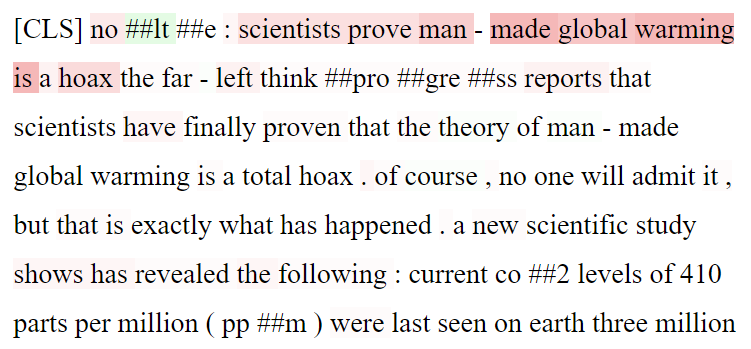
\includegraphics[width=\linewidth]{obrazky-figures/global_warming2.png}
      \caption{BERT model, correctly classified.}
      \label{fig:inter_anal1_a}
    \end{subfigure}%
    \begin{subfigure}{.5\textwidth}
      \centering
      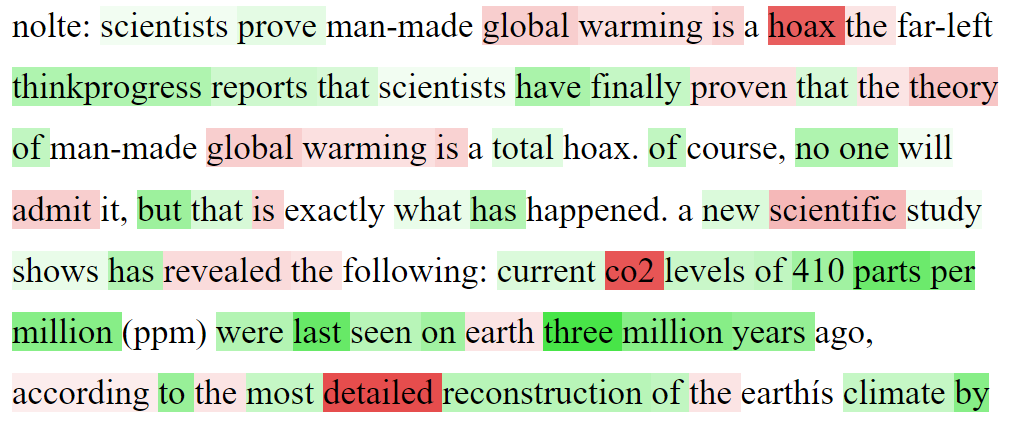
\includegraphics[width=\linewidth]{obrazky-figures/bayes_glob_warm.png}
      \caption{Baseline model, correctly classified.}
      \label{fig:inter_anal1_b}
    \end{subfigure}
    \caption{Visualization of interpretability for an unreliable article with a climate topic.}
    \label{fig:inter_anal1}
\end{figure}

Both models successfully classified the article claiming that global warming is a hoax as unreliable. A potential concern from this observation may be that the models would consider all articles about global warming as unreliable. To test this hypothesis figure \ref{fig:inter_anal2} shows the interpretation of a reliable article about global warming. The baseline model indeed classified the article as unreliable. The BERT model, on the other hand, correctly classified the article and identified \texttt{unesco} as a reliable entity.

\begin{figure}[H]
    \centering
    \begin{subfigure}{.5\textwidth}
      \centering
      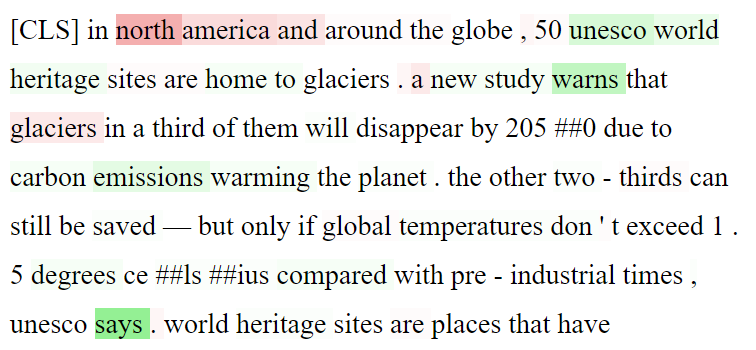
\includegraphics[width=\linewidth]{obrazky-figures/unesco_bert.png}
      \caption{BERT model, correctly classified.}
      \label{fig:inter_anal2_a}
    \end{subfigure}%
    \begin{subfigure}{.5\textwidth}
      \centering
      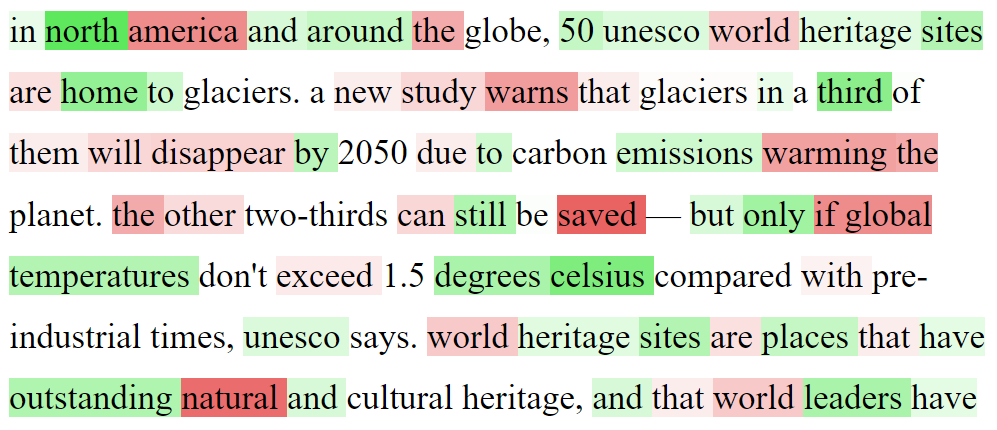
\includegraphics[width=\linewidth]{obrazky-figures/bayes_unecso.png}
      \caption{Baseline model, incorrectly classified.}
      \label{fig:inter_anal2_b}
    \end{subfigure}
    \caption{Interpretability of a reliable article with topic climate.}
    \label{fig:inter_anal2}
\end{figure}

As already noted in chapter \ref{experiments}, the baseline model considers all articles about football as reliable. Figure \ref{fig:inter_anal3} shows the visualization of interpretability for a reliable article about football. Both models correctly classified this article and identified football-related terms like \texttt{arsenal}, \texttt{title}, \texttt{scores}, and \texttt{match} as reliable. The baseline was influenced by the names of players and coaches --- e.g., \texttt{erling haaland}, \texttt{bruyne}, \texttt{pep} --- a lot more than the BERT model.

\begin{figure}[H]
    \centering
    \begin{subfigure}{.5\textwidth}
      \centering
      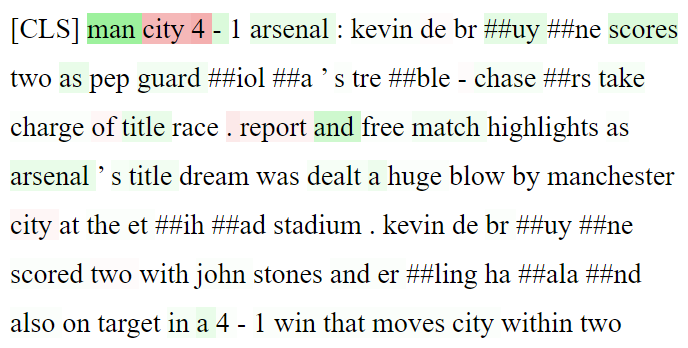
\includegraphics[width=\linewidth]{obrazky-figures/man-city.png}
      \caption{BERT model, correctly classified.}
      \label{fig:inter_anal3_a}
    \end{subfigure}%
    \begin{subfigure}{.5\textwidth}
      \centering
      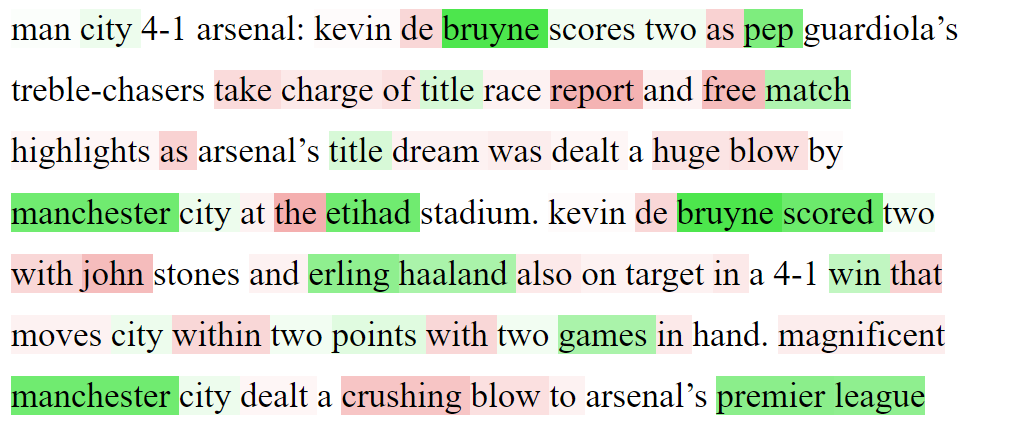
\includegraphics[width=\linewidth]{obrazky-figures/bayes_football1.png}
      \caption{Baseline model, correctly classified.}
      \label{fig:inter_anal3_b}
    \end{subfigure}
    \caption{Interpretability of a reliable article about football.}
    \label{fig:inter_anal3}
\end{figure}

Figure \ref{fig:inter_anal4} shows the interpretability of an unreliable article about football. This article is a fictional story about a reckless football player generated by ChatGPT. The BERT classifier managed to correctly identify it as unreliable as it uses a style similar to tabloid journalism that tries to shock readers through scandals and sensationalism. The baseline also identified the sensationalism in the article but still identified it as reliable because it contains the word \texttt{football}.

\begin{figure}[H]
    \centering
    \begin{subfigure}{.5\textwidth}
      \centering
      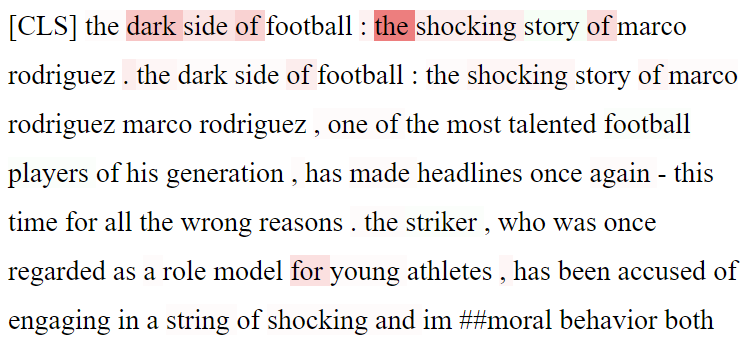
\includegraphics[width=\linewidth]{obrazky-figures/football_fake.png}
      \caption{BERT model, correctly classified.}
      \label{fig:inter_anal4_a}
    \end{subfigure}%
    \begin{subfigure}{.5\textwidth}
      \centering
      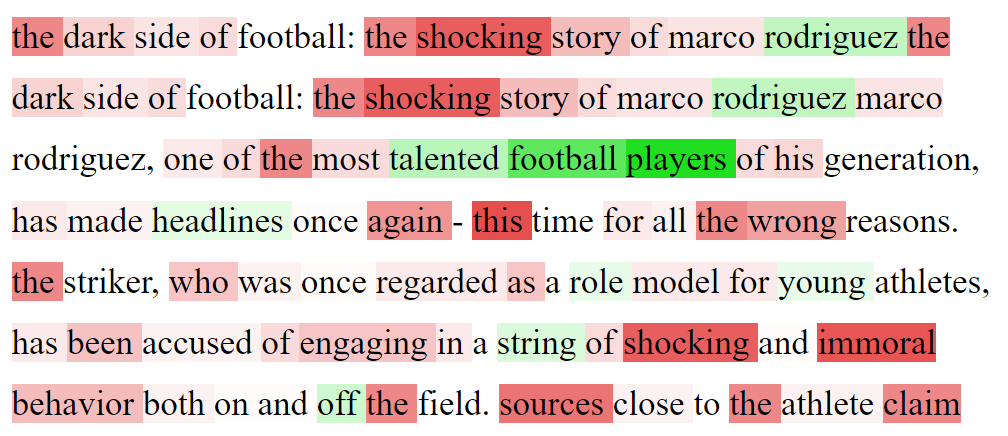
\includegraphics[width=\linewidth]{obrazky-figures/bayes_football2.png}
      \caption{Baseline model, incorrectly classified.}
      \label{fig:inter_anal4_b}
    \end{subfigure}
    \caption{Interpretability of an unreliable article about football generated by ChatGPT.}
    \label{fig:inter_anal4}
\end{figure}
 
Another hypothesis found in chapter \ref{experiments} is that the baseline is not able to correctly classify reliable scientific articles. Figure \ref{fig:inter_anal9} shows the interpretability of such an article. The baseline indeed failed to successfully classify this article. Science-based words like \texttt{nutrient}, \texttt{biomass}, \texttt{research}, \texttt{science} all have a negative contribution to the prediction. 

\begin{figure}[H]
    \centering
    \begin{subfigure}{.5\textwidth}
      \centering
      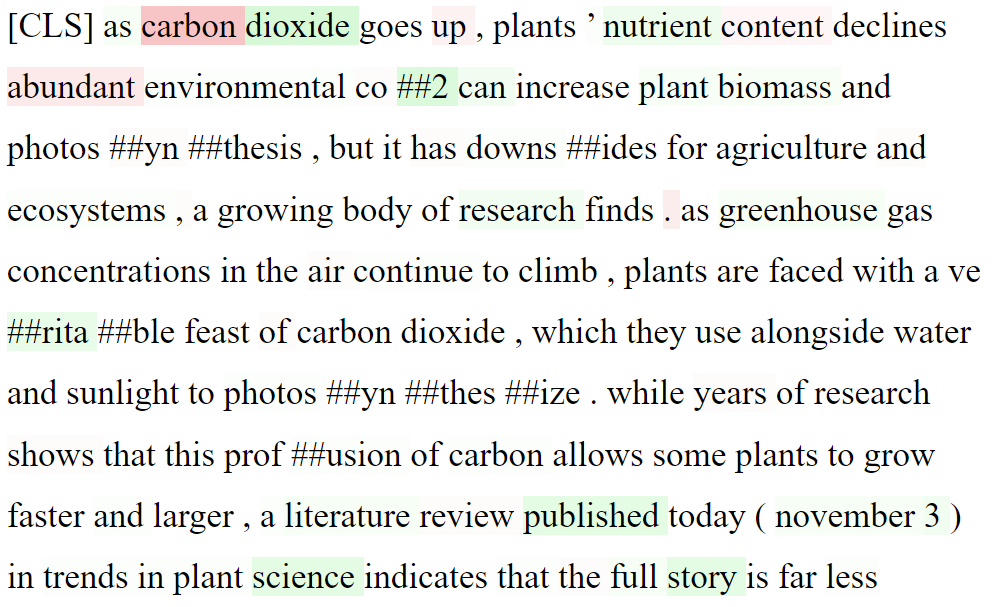
\includegraphics[width=\linewidth]{obrazky-figures/bert_science.png}
      \caption{BERT model, correctly classified.}
      \label{fig:inter_anal9_a}
    \end{subfigure}%
    \begin{subfigure}{.5\textwidth}
      \centering
      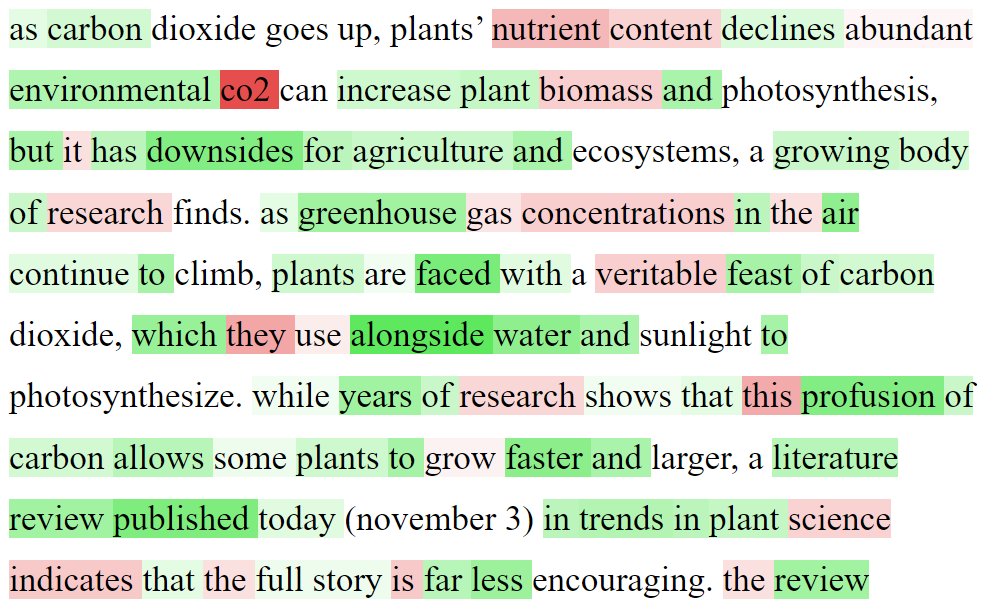
\includegraphics[width=\linewidth]{obrazky-figures/bayes_science.png}
      \caption{Baseline model, incorrectly classified.}
      \label{fig:inter_anal9_b}
    \end{subfigure}
    \caption{Interpretability of a reliable article about science.}
    \label{fig:inter_anal9}
\end{figure}

The BERT model, on the other hand, correctly classified the article as reliable. Figure \ref{fig:inter_anal6} shows a reliable article with the topic of war on which the BERT classifier failed. The cues discovered by the interpretation method seem confusing. On the second row, the word \texttt{reuters} is marked with red and later in the text the same word is green. It is important to note that this may be caused by a different context in each case, however, the interpretation of this article still remains slightly confusing.

\begin{figure}[H]
    \centering
    \begin{subfigure}{.5\textwidth}
      \centering
      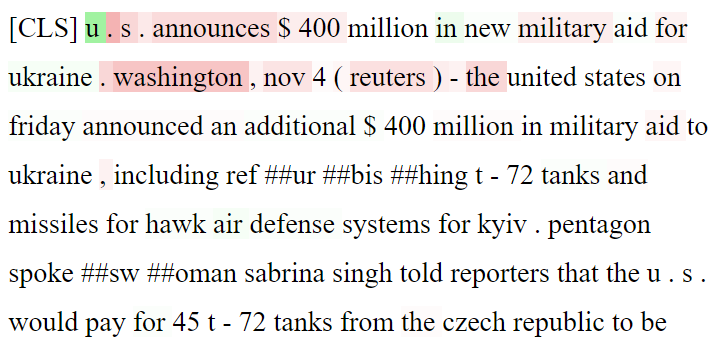
\includegraphics[width=\linewidth]{obrazky-figures/war_fail.png}
      \label{fig:inter_anal6_a}
    \end{subfigure}%
    \begin{subfigure}{.5\textwidth}
      \centering
      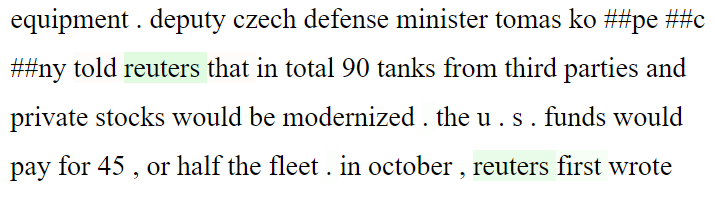
\includegraphics[width=\linewidth]{obrazky-figures/war_fail_reuters.png}
      \label{fig:inter_anal6_b}
    \end{subfigure}
    \caption{Example of a reliable article with the topic of war incorrectly classified by the BERT model as unreliable.}
    \label{fig:inter_anal6}
\end{figure}

Besides using the articles from the FNI dataset, the interpretability was also analysed using one source from the NELA dataset the \texttt{truth theory}. As described in table \ref{tab:bert_acc_per_src} in section \ref{sec:accuracy_per_source}, this reliable source obtained the lowest accuracy of only 19\% from the BERT model. Figure \ref{fig:truth_disc1} shows the interpretability of two articles by this source. 


\begin{figure}[H]
    \centering
    \begin{subfigure}{.5\textwidth}
      \centering
      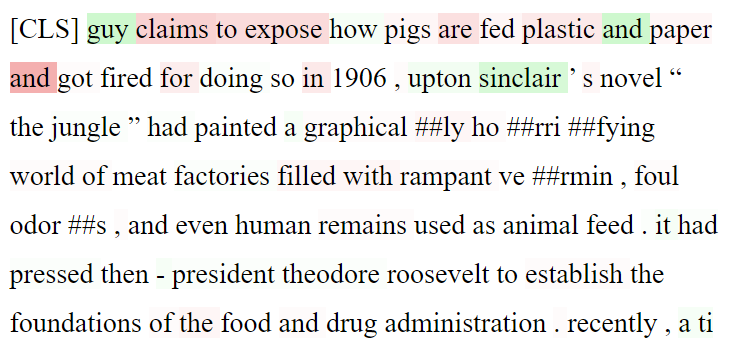
\includegraphics[width=\linewidth]{obrazky-figures/truth-theory1.png}
      \caption{BERT model}
      \label{fig:truth_disc_1a}
    \end{subfigure}%
    \begin{subfigure}{.5\textwidth}
      \centering
      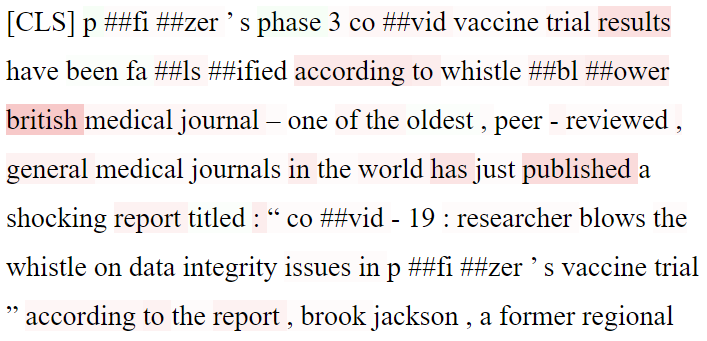
\includegraphics[width=\linewidth]{obrazky-figures/truth-theory3.png}
      \caption{BERT model}
      \label{fig:truth_disc_1b}
    \end{subfigure}
    \caption{Reliable articles by source \texttt{truth theory} classified as unreliable.}
    \label{fig:truth_disc1}
\end{figure}

The \texttt{truth theory} is a source marked as reliable on the MBFC webpage with a high factuality score. After analysing its articles, however, it seemed that the articles are written in a way that resembles fake news and tabloid journalism. Using phrases like \texttt{guy claims to expose how pigs are fed plastic} or \texttt{covid vaccine trial results falsified} really resembles unreliable sources. This source is therefore considered to be an edge case as all the other sources achieved much better accuracy. However, there are also some articles by this source that seem to be reliable and were incorrectly classified. One of these examples is shown in figure \ref{fig:truth_disc2}. In this case, the interpretability is also rather confusing.

\begin{figure}[H]
    \centering
    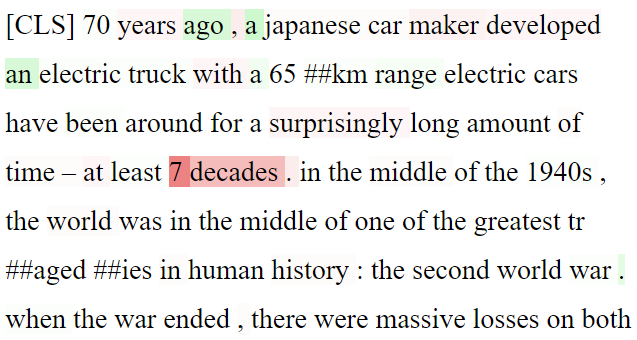
\includegraphics[scale=0.6]{obrazky-figures/truth-theory4.png}
    \caption{Confusing interpretability of a reliable article by source \texttt{truth theory} incorrectly classified by the BERT model as unreliable.}
    \label{fig:truth_disc2}
\end{figure}

Overall the interpretability methods of both classifiers work better on unreliable articles where they are able to identify sensational and shocking headlines. Naturally, it is easier to show that an article is fake rather than prove that it is true. In many reliable articles, the interpretability was not self-explanatory even though the article was correctly classified. A manual analysis of 30 articles showed that the interpretability method of the BERT classifier worked well for 80\% of unreliable and 47\% of reliable articles.



\chapter{Predicting the Credibility of Sources}
\label{chap:source_credibility}
The classifiers implemented in this thesis are constructed to predict the credibility of articles. The goal of this chapter is to find out whether it is possible to use the predicted credibility of articles obtained from the BERT classifier to predict the credibility of media sources. To evaluate the credibility of sources, two different methods were implemented. The first method uses the average credibility of articles published by the given source. The second method creates embeddings from the predicted credibilities of articles and uses them to train a logistic regression model that learns to predict the credibility of sources.
To evaluate these two approaches, the results are compared with ground truth labels and with a state-of-the-art method which uses graph-neighbourhood exploitation algorithms. Following is the explanation of these methods.


\section{Graph-neighborhood Exploitation Method}
The credibility of sources used as the reference for the other two methods was obtained from a method based on graph-neighbourhood exploitation. This method was implemented by Sergio Burdisso (sergio.burdisso@idiap.ch) who kindly shared his results for the purpose of this thesis. As of now, the method has not been officially published and is therefore described only briefly. The method uses citations and references to other sources mentioned in articles to construct a graph, where the nodes represent the sources and the edges represent their relationship based on the citations. Based on this graph it uses reinforcement learning techniques to identify reliable and unreliable sources and compute their credibility. 

The author used 4497 sources crawled from the MBFC website and annotated their reliability following the policy described in the NELA-GT-2019 paper. Each source is assigned a value from $[-1, 1]$ that represents its credibility. These values were transformed to range $[0,1]$ to match the probabilities used by the BERT classifier. Out of the 4497 sources, only 88 were present in the dataset used in this thesis (57 reliable, 31 unreliable). Therefore, these 88 common sources are used to compare the computed credibilities. The following sections describe the methods implemented in this thesis.


\pagebreak

\section{Average Credibility Method}
The first method computes the credibility of a source simply as the average reliability of all articles published by the given source. The articles of the source are all evaluated by the BERT classifier. For each article, the classifier outputs the probabilities of two classes (\texttt{reliable} and \texttt{unreliable}). The probability of the \texttt{reliable} class is used to compute the average. Therefore, the reliability of a source is computed as the average reliability of its articles, predicted by the BERT classifier. Figure \ref{fig:avg_rel} shows a graphical representation of this method.

\begin{figure}[H]
    \centering
    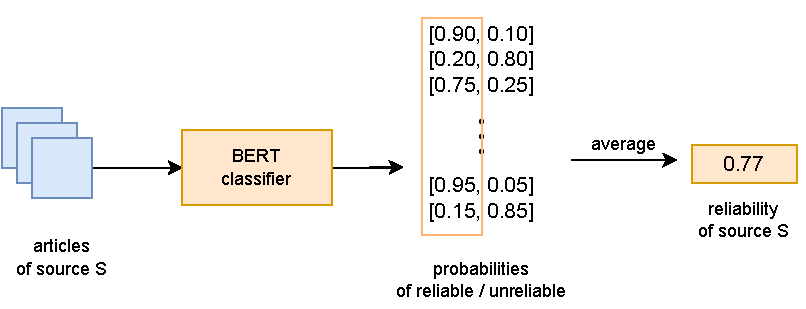
\includegraphics[scale=0.9]{obrazky-figures/avg_reliability.pdf}
    \caption{Computing the reliability of source $S$ using the average reliability method.}
    \label{fig:avg_rel}
\end{figure}


\section{Embedding Method}
The second method uses the probabilities of class \texttt{reliable} predicted by the BERT classifier to create embeddings. All articles are first evaluated by the BERT classifier and the output probabilities of class \texttt{reliable} are sorted in descending order. Then $k$ highest and $k$ lowest values of the predicted reliability are concatenated to create a $2k$-dimensional embedding vector. This vector is then used to train a logistic regression model, which consists of one linear layer with a sigmoid activation function, to predict the reliability of the source based on its embedding. Figure \ref{fig:embeddings} shows the construction of the embedding for source $S$. 

\begin{figure}[H]
    \centering
    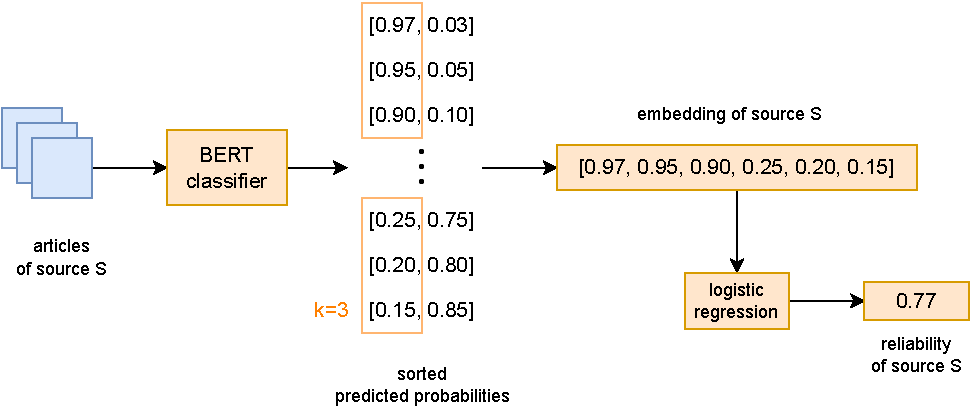
\includegraphics[scale=0.9]{obrazky-figures/embedding.pdf}
    \caption{Computing the reliability of source $S$ using the embedding method with logistic regression for $k=3$.}
    \label{fig:embeddings}
\end{figure}

The embedding vectors often contained very small numbers (e.g., 1.1166e-04, 1.7239e-05, etc.) among the $k$ lowest reliabilities. These numbers are interpreted as zeros by the logistic regression model which made the learning difficult. Normalizing the vector with the L2 norm did not show any improvement nor did applying mean removal. The problem was finally solved by scaling all values of the vector by 10,000. Different values of $k$ were tried and evaluated by comparing the resulting reliabilities of sources with the referential values. The following section discusses the results in detail.

% \begin{figure}[H]
%     \centering
%     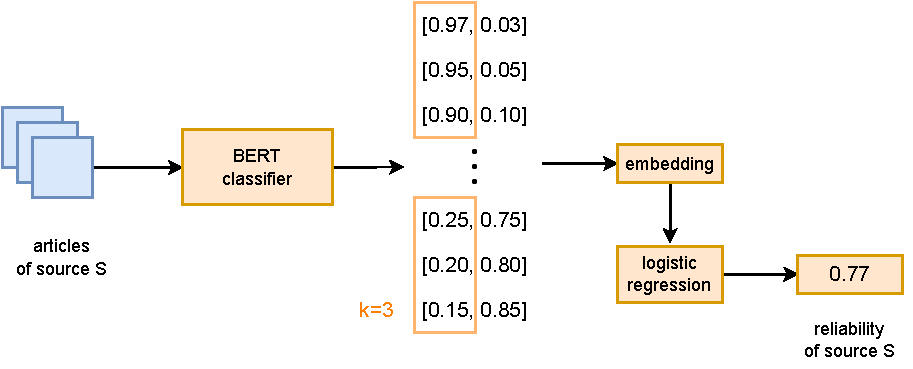
\includegraphics[scale=0.9]{obrazky-figures/emb_log_reg.pdf}
%     \caption{Computing the reliability of sources using the logistic regression method with embeddings.}
%     \label{fig:log_reg}
% \end{figure}

\section{Comparing the Results}
The implemented methods are evaluated by comparing their results with ground truth labels and the referential scores obtained from the graph-neighbourhood method. Both methods were trained on the articles from the NELA test set. The test set contains 249 sources and 88 of them are also present in the referential scores. Therefore these 88 sources were only used for evaluation, not for training of the average reliability and embedding methods. To compare the computed reliabilities with the referential scores the Jensen-Shannon distance and Kendall rank methods are used. 

\subsection*{Jensen–Shannon Divergence}
The Jensen–Shannon (JS) divergence, presented in \cite{js_divergence}, is based on the Kullback-Leibler (KL) divergence. The KL divergence score quantifies how much one probability distribution differs from another probability distribution. The KL divergence between two distributions $P$ and $Q$ is computed using the following equation.

\begin{equation}
    KL(P || Q) = \sum_{x \in X} P(x) \cdot \operatorname{log}\frac{P(x)}{Q(x)}
    \label{eq:kl_divergence}
\end{equation}

where $P(x)$ and $Q(x)$ are the probabilities of $x$ in distributions $P$ and $Q$. The KL divergence is not symmetric as $KL(P||Q) \neq KL(Q||P)$. The Jensen-Shannon (JS) divergence uses the KL divergence to calculate a normalized score that is symmetrical. The computation of JS divergence is described by equation \ref{eq:js_divergence}. 

\begin{equation}
    JS(P||Q) = \frac{1}{2} \cdot KL(P||M) + \frac{1}{2} \cdot KL(Q||M) 
    \label{eq:js_divergence}
\end{equation}

where $M = \frac{1}{2} (P+Q)$. The JS divergence computes symmetrical values --- meaning $JS(P||Q) = JS(Q||P)$ --- ranging from 0 (distributions $P$ and $Q$ are identical) to 1 (biggest difference) when using the base-2 logarithm. Finally, the JS distance used in this thesis is simply the square root of the JS divergence.

\begin{equation}
    JS_{distance}(P||Q) = \sqrt{JS(P||Q)}
    \label{eq:js_distance}
\end{equation}

\subsection*{Kendall Rank Correlation Coefficient (Tau)}
The second metric used for comparing the results is the Kendall rank correlation coefficient, also known as the Kendall tau. This method is used when the compared variables are ordinal or ranked data. It measures the strength of the association between two variables and the direction of the relationship. The computation of Kendall tau is based on the appearance of concordant and discordant pairs in the data. Imagine we compare two columns of ranked data $X$ and $Y$. A pair of observations $(x_i, y_i)$ and $(x_j, y_j)$ where $i < j$ are concordant when the following statement is true:

$$(x_i > x_j) \wedge (y_i > y_j) \quad \lor \quad (x_i < x_j) \wedge (y_i < y_j)$$

otherwise, the pairs of observations are considered discordant. The number of concordant and discordant pairs between $X$ and $Y$ is counted and used to compute the rank. Several versions of the Kendall tau exist. In this thesis, the tau-b version is used as it accounts for ties in the columns. The Kendall tau-b uses the following equation\footnote{\url{https://docs.scipy.org/doc/scipy-0.15.1/reference/generated/scipy.stats.kendalltau.html}}:

\begin{equation}
    \tau_b = \displaystyle{\frac{P - Q}{\sqrt{((P+Q+T) \cdot (P+Q+U))}}}
\end{equation}

where $P$ is the number of concordant pairs, $Q$ is the number of discordant pairs, $T$ is the number of ties in $X$ and $U$ is the number of ties in $Y$. If a tie occurs for the same pair in both $X$ and $Y$, it is not added to either $T$ or $U$. The value of Kendall tau ranges from -1 to 1. The closer to 0 the lower the association between $X$ and $Y$. The further from 0 the bigger is the association. The negative sign only indicates the direction of the relationship. 

Table \ref{tab:js_kt_resluts} shows the results of JS distance and Kendall tau of the two methods (using the BERT classifier and average reliability/embeddings) compared with the referential reliability scores of sources obtained from the graph-neighbourhood method. Both methods obtained values around 0.2 for the JS distance (where 0 indicates identical distributions and 1 indicates the biggest difference). The embedding method outperformed the average reliability in both metrics, however for different values of $k$. It achieved the best tau value of 0.63 for $k=22$ and the best JS distance for $k=4$.

\begin{table}[H]
    \centering
\begin{tabular}{|c|c|c|}
\hline
\textbf{Method} & \textbf{JS distance} & \textbf{Kendall tau} \\ \hline
avg reliability & 0.21                 & 0.51                 \\ \hline
embeddings (k=4)      & 0.20                 & 0.56                 \\ \hline
embeddings (k=22)     & 0.25                 & 0.63                 \\ \hline
\end{tabular}
    \caption{Results of JS distance and Kendall tau of the average reliability and embedding methods compared with the referential values.}
    \label{tab:js_kt_resluts}
\end{table}

Figure \ref{fig:tau_js_vs_k} shows the Kendall tau and JS distance of the embedding method for different values of $k$ from 1 to 30. The value of $k$ represents how many article reliability scores are used to create the embedding. It also influences the required number of articles for each source, e.g., when $k=10$ all sources must contain at least 20 articles to create the embedding. In cases where the source contains fewer articles than is required, the embedding uses zeros as padding at the end. A growing tendency can be seen in figure \ref{fig:tau_vs_k}, indicating that the logistic regression method improved with longer embeddings. It is interesting to see that with the growing value of $k$ the tau value is improving whereas the JS distance deteriorates. The change in JS distance, however, is not as significant as all values are between 0.2 and 0.26. On the other hand, the tau value managed to improve from 0.45 to 0.63. Therefore it seems that a bigger number of embeddings improves the ordering of the computed reliability, but the accuracy of the scores remains approximately the same. 

\begin{figure}[H]
    \centering
    \begin{subfigure}{.5\textwidth}
      \centering
      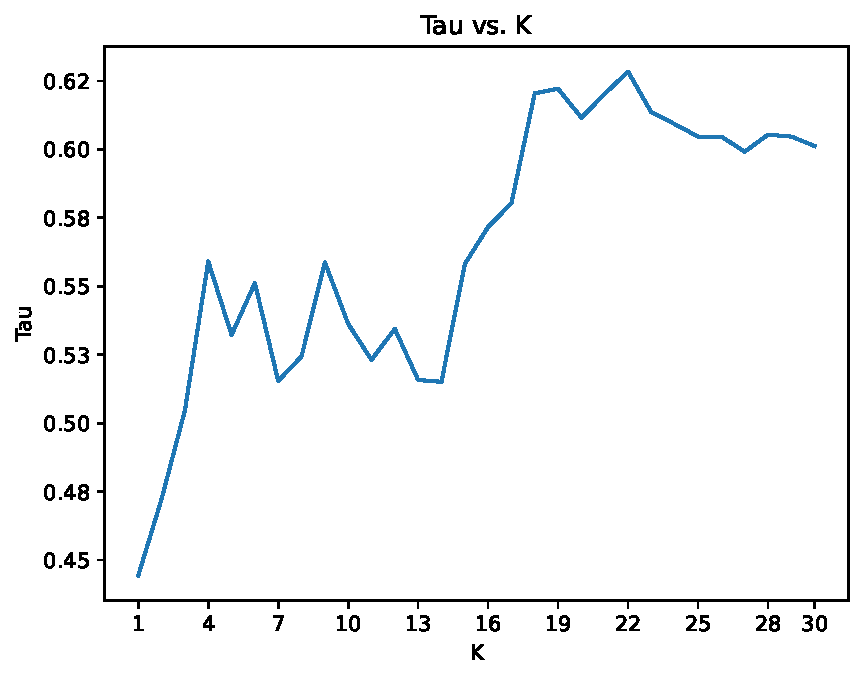
\includegraphics[width=\linewidth]{obrazky-figures/tau_vs_k30.pdf}
      \caption{}
      \label{fig:tau_vs_k}
    \end{subfigure}%
    \begin{subfigure}{.5\textwidth}
      \centering
      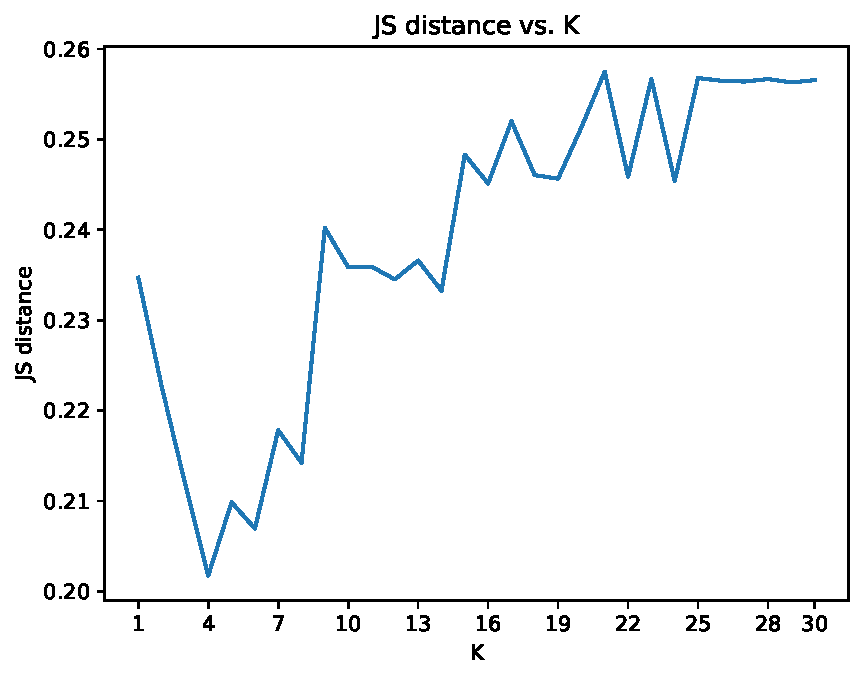
\includegraphics[width=\linewidth]{obrazky-figures/js_vs_k30.pdf}
      \caption{}
      \label{fig:js_vs_k}
    \end{subfigure}
    \caption{Kendall tau and JS distance of the embedding method based on the value of $k$.}
    \label{fig:tau_js_vs_k}
\end{figure}

To see how the values of tau and JS vary, they were computed separately for four groups of sources. Each group is chosen randomly and contains around 20 sources. The results for the embedding method with $k=22$ are displayed in figure \ref{fig:tau_vs_k_groups}.

\begin{figure}[H]
    \centering
    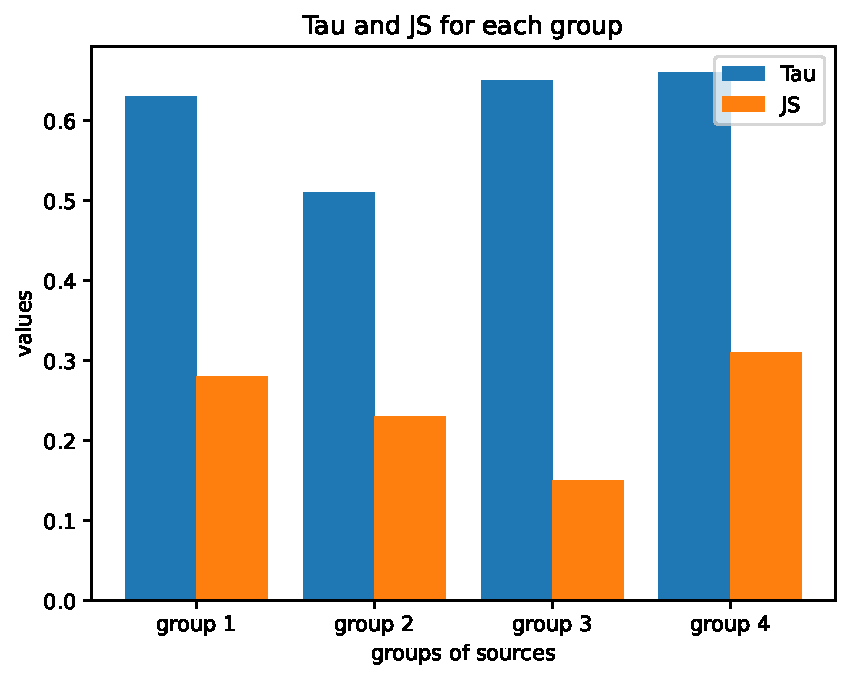
\includegraphics[scale=0.6]{obrazky-figures/tau_js_groups.pdf}
    \caption{Kendall tau and JS distance of the embedding method with $k=22$ for different groups of approximately 20 sources.}
    \label{fig:tau_vs_k_groups}
\end{figure}

Besides comparing the computed source reliabilities with the referential scores they were also compared with the ground truth labels. Figure \ref{fig:accuracy_vs_threshold} shows the accuracy of both methods for different values of threshold. The threshold is used to determine the label of a source based on the computed reliability score. If the score is higher than the selected threshold the source is considered reliable, otherwise it is considered as unreliable. An interesting observation is that the accuracy is above 90\% for most of the threshold values. This is explained when looking at the average predicted score for each label. Unreliable sources have an average predicted score of 0.07 and reliable sources have an average score of 0.93 (for the average probability method). Still, the best threshold value was found to be 0.6 as it performs the best for all approaches.

\begin{figure}[H]
    \centering
    \begin{subfigure}{.5\textwidth}
      \centering
      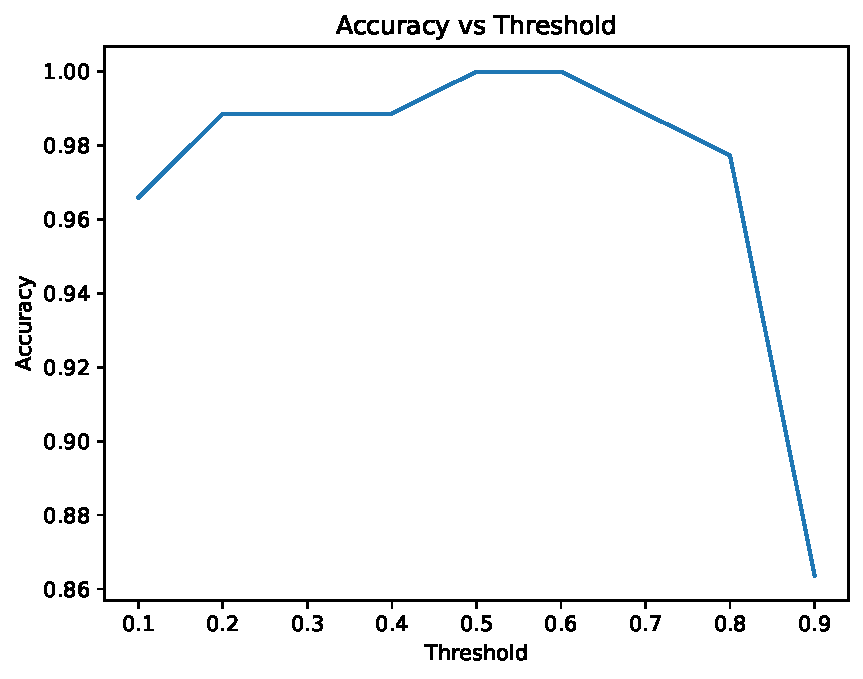
\includegraphics[width=\linewidth]{obrazky-figures/accuracy_vs_threshold_avg.pdf}
      \caption{Average credibility method.}
      \label{fig:accuracy_vs_logreg}
    \end{subfigure}%
    \begin{subfigure}{.5\textwidth}
      \centering
      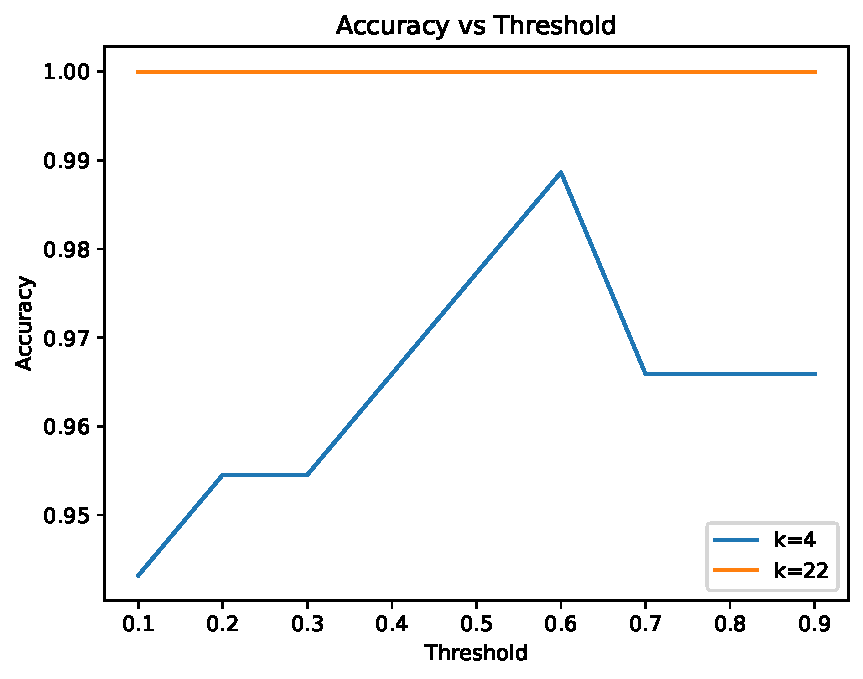
\includegraphics[width=\linewidth]{obrazky-figures/accuracy_vs_threshold_logreg.pdf}
      \caption{Embedding method.}
      \label{fig:accuracy_vs_avg}
    \end{subfigure}
    \caption{Accuracy of the embedding and average credibility methods for different thresholds.}
    \label{fig:accuracy_vs_threshold}
\end{figure}


The conclusion of this experiment is therefore that a classifier computing reliability scores of articles based only on text can be used to assess the reliability of media sources on the internet.



%%%%%%%%%%%%%%%%%%%%%%%%%%%%%%%%%%
% Conclusion
\chapter{Conclusion}
\label{conclusion}
The goal of this thesis was to study the biases and cues exploited by content-based methods in the text of fake news articles and evaluate their performance on predicting the reliability of articles and media sources. The first step was to define the problem of fake news detection and study the methods and previous work in this area. After that, a comprehensive analysis of available datasets was conducted. Each dataset was evaluated for its qualities and suitability for this thesis.

The most suitable dataset was found to be the NELA-GT-2021 dataset and was therefore used to train the classifiers in this thesis. This dataset was preprocessed by extending the source-level labels (indicating the reliability of sources) to article-level labels as each article obtained the label of its source. Another preprocessing step was filtering keywords from the dataset (e.g., names of sources and specific terms) that would provide simple clues for the classifiers making them base the predictions on simple clues rather than actually understanding the text.
Another two datasets were created for testing and analysis. The first one called the Merged dataset, was formed by merging three fake news datasets with article-level labels and was used for further evaluation of the classifiers. The second dataset called the Fake News Interpretability (FNI) dataset, was created by the author of this thesis. It consists of 46 manually collected articles (23 reliable and 23 unreliable) from various sources on the internet. Each article is assigned a topic that reflects what is its content related to. The topics of the articles were used to analyse the performance of the classifiers in different areas.

For the implementation of the classifiers, two different methods were selected. The first method implements the baseline model and is based on TF-IDF and a Multinomial Naive Bayes classifier. The second method intended to improve the baseline uses the BERT transformer. 
Both classifiers were evaluated on a test split of the NELA dataset, the Merged dataset and the FNI dataset. The analysis revealed several strengths and weaknesses of both classifiers. The baseline was not very successful in classifying reliable articles. It achieved a very low accuracy of only 48\% on articles with a pro-science bias (science-based articles using credible scientific sourcing) as well as on articles with a very high factuality score (62\% accuracy). The average accuracy per source for unreliable articles was 83\% whereas for reliable articles only 71\%. The baseline was also not able to identify unreliable articles about football as it learned to connect football-related terms with a sign of reliability.
The BERT classifier managed to outperform the baseline in every aspect and mitigated its disabilities. The difference between the average accuracy per source for unreliable and reliable articles was not so significant (only 3\%). The BERT classifier performed much better in classifying the pro-science articles (94\% accuracy) and articles with a very-high factuality (97\% accuracy). The BERT classifier also managed to identify fake articles about football, a topic considered reliable by the baseline. Among the limitations of the implemented classifiers can be the fact that both methods can be used only for text and cannot be applied to other types of media (e.g., video, images, etc.).

For the BERT classifier, a method of interpretability based on Integrated gradients was implemented. The interpretability was analysed using articles from the FNI dataset and one reliable source from the NELA dataset that achieved the lowest accuracy. This reliable source with a high factuality score achieved an accuracy of only 19\%. After analysing its articles it seemed like the source often uses shocking headlines and style-of-writing similar to unreliable articles. The interpretability method worked better for unreliable articles and was able to identify the shocking headlines they often use. For reliable articles, the results were often inconsistent. A manual analysis of 30 articles showed that the Integrated gradients method worked well for 80\% of unreliable and 47\% of reliable articles.

The implemented classifiers were also evaluated for their ability to predict the reliability of sources using the computed reliability of their articles. Two methods were created and their results were compared with referential values obtained from a state-of-the-art method using graph exploitation. The results showed that a classifier constructed to compute the reliability of articles can be successfully applied to media sources. 

This thesis succeeded in creating a functional classifier for predicting the credibility of articles and sources on the internet using only the text of articles. The method of interpretability performed well in identifying the sensationalism used in fake articles but showed uncertainty in identifying reliability. A more complex method could be applied in future work, e.g., a masker neural network inspired by the masker model in \cite{claim-dissector} —-- a model that learns to mask the least number of tokens to change the decision of the classifier, where the tokens that were masked represent the most important tokens for the decision. The content-based classifier created in this thesis could further be applied to downstream tasks, e.g., to improve an existing fact-checking model by assigning reliability to the documents used as evidence.